\documentclass[%
master,      % тип документа
natbib,      % использовать пакет natbib для "сжатия" цитирований
subf,        % использовать пакет subcaption для вложенной нумерации рисунков
href,        % использовать пакет hyperref для создания гиперссылок
colorlinks,  % цветные гиперссылки
%fixint,     % включить прямые знаки интегралов
]{disser}

\usepackage[
a4paper, mag=1000,
left=3cm, right=1cm, top=2cm, bottom=2cm, headsep=0.7cm, footskip=1cm
]{geometry}

\usepackage{natbib}
\usepackage[intlimits]{amsmath}
\usepackage{amssymb,amsfonts}

\usepackage[T2A]{fontenc}
\usepackage[utf8]{inputenc}
\usepackage[english,russian]{babel}
\ifpdf\usepackage{epstopdf}\fi
\usepackage[autostyle]{csquotes}

\usepackage[singlelinecheck=false]{caption}
\usepackage{cmap}
\usepackage{cancel}

%\usepackage[document]{ragged2e}
\pretolerance=10000
%\sloppy

% Шрифт Times в тексте как основной
%\usepackage{tempora}
% альтернативный пакет из дистрибутива TeX Live
\usepackage{cyrtimes}

% Шрифт Times в формулах как основной
%\usepackage[varg,cmbraces,cmintegrals]{newtxmath}
% альтернативный пакет
\usepackage[lite]{mtpro2}
\pdfmapfile{mtpro2.map}

% Список сокращений и условных обозначений
\usepackage[intoc,nocfg,russian]{nomencl}
\newcommand{\nomencl}[2]{#1 --- #2\nomenclature{#1}{#2}}
\setlength{\nomlabelwidth}{3em}
\setlength{\nomitemsep}{-\parsep}
\renewcommand{\nomlabel}[1]{#1 ---}
\makenomenclature

% Плавающие рисунки "в оборку".
\usepackage{wrapfig}

% Номера страниц снизу и по центру
\pagestyle{footcenter}
\chapterpagestyle{footcenter}

% Точка с запятой в качестве разделителя между номерами цитирований
%\setcitestyle{semicolon}

% Использовать полужирное начертание для векторов
\let\vec=\mathbf

% Включать подсекции в оглавление
\setcounter{tocdepth}{2}

\usepackage{graphicx}
\graphicspath{{pictures/}}

\captionsetup[figure]{justification=centering}
\captionsetup[table]{position=top,aboveskip=5pt}

% Покдлючить пакет с возможностью подсчета станиц, рисунков, формул, таблиц и т.д.
%\usepackage{totcount}
%\regtotcounter{page}
%\newtotcounter{mfigure}
%\newtotcounter{mequation}
%\newtotcounter{mtable}
%\newtotcounter{bibcnt}
%
%\def\oldfigure{} \let\oldfigure=\figure
%\def\figure{\stepcounter{mfigure}\oldfigure}
%
%\def\oldequation{} \let\oldequation=\equation
%\def\equation{\stepcounter{mequation}\oldequation}
%
%\def\oldtable{} \let\oldtable=\table
%\def\table{\stepcounter{mtable}\oldtable}
%
%\def\oldbibitem{} \let\oldbibitem=\bibitem
%\def\bibitem{\stepcounter{bibcnt}\oldbibitem}
%
%\makeatletter
%\setlength{\parindent}{7.5ex}
%\renewcommand{\tocprethechapter}{}
%\renewcommand{\tocpostthechapter}{}
%\renewcommand{\tocpostthesection}{}
%\renewcommand{\postthesection}{\ }
%\renewcommand{\tocsectionindent}{0em}
%\renewcommand{\tocsectionnameindent}{1.5em}
%\renewcommand{\sectionindent}{10em}
%\renewcommand{\captionlabeldelim}{\textendash}
%\renewcommand{\thetable}{\@arabic\c@table}
%\renewcommand{\theequation}{\@arabic\c@equation}
%\renewcommand{\fnum@figure}{Рисунок \thefigure}
%\renewcommand{\labelitemi}{\textendash}
%\makeatother
%
%\DeclareCaptionFormat{plain}{\captionlabelfont #1 \captionlabeldelim \ #3 \par}
%
%\makeatletter
%\renewcommand*\l@chapter[2]{%
%\ifnum \c@tocdepth >\m@ne
%%\addpenalty{-\@highpenalty}
%\vskip 1.0em \@plus\p@
%%\setlength\@tempdima{4.5em}
%\begingroup
%\parindent \z@ \rightskip \@pnumwidth
%\parfillskip -\@pnumwidth
%%\leavevmode\tocchapterfont
%\advance\leftskip\@tempdima
%\hskip -\leftskip
%#1\nobreak
%\tocchapterfillfont\tocchapterfill\hfill
%\nobreak\hb@xt@\@pnumwidth{\hss\tocchapternumfont #2}\par
%\penalty\@highpenalty
%\endgroup
%\fi}
%\makeatother
%
%\makeatletter
%\renewcommand{\@makechapterhead}[1]{% Начало макроопределения
%\vspace*{20 pt}% Пустое место вверху страницы
%{\parindent=0pt
%\hspace{1.5 cm}
%\upshape \mdseries \rmfamily \normalsize \large
%\thechapter \hspace{2 pt} #1\par % заголовок главы
%\nopagebreak
%\vspace{5 pt}
%}
%}
%\makeatother
%
%\renewcommand{\sectionfont}{\upshape \mdseries \rmfamily \normalsize \large}
%\renewcommand{\sectionindent}{1.6 cm}

\begin{document}

    % Переопределение стандартных заголовков
%    \def\introname{\upshape \mdseries \rmfamily \normalsize \large ВВЕДЕНИЕ}
%    \def\contentsname{\upshape \mdseries \rmfamily \normalsize \large СОДЕРЖАНИЕ}
%    \def\conclusionname{\upshape \mdseries \rmfamily \normalsize \large ЗАКЛЮЧЕНИЕ}
%    \def\bibname{\upshape \mdseries \rmfamily \normalsize \large СПИСОК ИСПОЛЬЗОВАННЫХ ИСТОЧНИКОВ}

    %
    % Титульный лист на русском языке
    %

%    \institution{Название организации}
%
%    % Имя лица, допускающего к защите (зав. кафедрой)
%    \apname{ФИО зав. кафедрой}
%
%    \title{ДИССЕРТАЦИЯ\\[-14pt]на соискание ученой степени\\МАГИСТРА}
%
%    \topic{Тема диссертации}
%
%    % Автор
%    \author{ФИО автора}
%    % Группа
%    \group{1111/1}
%    % Номер направления
%    \coursenum{111111}
%    \course{Название направления}
%    % Номер магистерской программы
%    \masterprognum{111111}
%    \masterprog   {Название программы}
%
%    % Научный руководитель
%    \sa      {ФИО руководителя}
%    \sastatus{д.~ф.-м.~н., ст.~н.~с.}
%    % Второй научный руководитель
%    %\sasnd      {ФИО руководителя}
%    %\sasndstatus{д.~ф.-м.~н., ст.~н.~с.}
%
%    % Рецензент
%    \rev      {ФИО рецензента}
%    \revstatus{д.~ф.-м.~н., в.~н.~с.}
%    % Второй рецензент
%    %\revsnd      {ФИО рецензента}
%    %\revsndstatus{д.~т.~н., ст.~н.~с.}
%
%    % Консультант
%    \con{ФИО консультанта}
%    \conspec{вопросам\\охраны труда}
%    \constatus{к.~т.~н., доц.}
%    % Второй консультант
%    %\consnd{ФИО консультанта}
%    %\consndspec{экономическим\\вопросам}
%    %\consndstatus{к.~э.~н., доц.}
%
%    % Город и год
%    \city{Санкт-Петербург}
%    \date{\number\year}
%
%    \maketitle

    %%
    %% Titlepage in English
    %%
    %
    %\institution{Name of Organization}
    %
    %% Approved by
    %\apname{Professor S.\,S.~Sidorov}
    %
    %\title{Master's Thesis}
    %
    %% Topic
    %\topic{Dummy Title}
    %
    %% Author
    %\author{Author's Name} % Full Name
    %\course{Physics} % Specialization
    %
    %\group{} % Study Group
    %\masterprog   {Title of program}
    %
    %% Scientific Advisor
    %\sa       {I.\,I.~Ivanov}
    %\sastatus {Professor}
    %
    %% Reviewer
    %\rev      {P.\,P.~Petrov}
    %\revstatus{Associate Professor}
    %
    %% Consultant
    %\con{}
    %\conspec{}
    %\constatus{}
    %
    %% City & Year
    %\city{Saint Petersburg}
    %\date{\number\year}
    %
    %\maketitle[en]

    % Реферат для НИР
%    %! Author = jaroslav
%! Date = 22.04.20
%\begin{titlepage}
%    \tiny
%    \scriptsize
%    \footnotesize
%    \small
%    \normalsize
%    \large
%    \Large
%    \LARGE
%    \huge
%    \Huge
%    \begin{center}
%        \large
%        РЕФЕРАТ
%    \end{center}
%
%    Отчет \total{page} страницы, %\total{mequation} формул,
%    \total{mfigure} рисунков,
%    \total{mtable} таблиц, \total{bibcnt} источников,
%
%    \hspace{0.5cm}ТЕОРИЯ ПРИНЯТИЯ РЕШЕНИЙ, ЭКСПЕРИМЕНТ ЭЛЛСБЕРГА,
%
%    \hspace{0.5cm}ОШИБКА КОНЪЮНКЦИИ, ЭФФЕКТ ДИЗЪЮНКЦИИ,
%
%    \hspace{0.5cm}ИНТЕРНЕТ РЕСУРСЫ, ДИЛЕММА ЗАКЛЮЧЕННОГО
%
%    Объектом исследования является модель социально-значимых Интернет
%    ресурсов, которое рассматривает отношения между индивидами в рамках
%    дискусси на популярном Интернет площадке.
%
%    Целью данной работы является поиск связей между моделью социально-
%    значимых Интернет ресурсов и экспериментами, объяснение которых
%    простыми моделями не представляется возможным.
%    Выявление этих связей позволит узнать возможные пути объяснения
%    этих эффектов, а также предсказать возможные другие когнитивные
%    эффекты.
%
%    В результате работы была вывлена связь между экспериментами и
%    моделью социально-значимых Интернет ресурсов
%
%    В дальнейшем, эта работа позвоит выявить связь между моделью
%    социально-значимых Интернет ресусов и квантово-подобным моделями
%    приянтия решений в условиях неопределенности
%\end{titlepage}

    % Содержание
    \tableofcontents

    % Введение
    %! Author = jaroslav
%! Date = 22.04.20
\intro

Современная наука хорошо справляется с естественнонаучными задачами окружающего мира.
Разработаны теории, модели которые хорошо описывают основные законы физики, химии, биологии.
И только к началу двадцатого века, ученые пришли к решению когнитивых задач.
Конечно, ранее эти задачи тоже изучались, но не так интенсивно и обсуждались лишь в
кругах филосовских мыслителей.
Такое позднее изучение когнитивных задач связано, конечно же, со сложностью формулировки,
постановкой экспериментов и малой применимостью результатов.
В современное время, необходимость в изучении когнитивных наук стало весомее из-за различных
эффектов с ошибками выбора правильного решения, развития задач искусственного интелекта,
изменений социальных отношений в современном обществе.
Как и любая другая наука, когнитивные задачи имеют свои парадоксы, которые сложно объяснить
простыми словами или законами.
В таком случае необходимо подбирать решения используя уже известные науке интрументы.
В данной работе такими инструментами являются теория графов и математический формализм.

    % Глава 1
    %! Author = jaroslav
%! Date = 20.03.20
\chapter{ЛИТЕРАТУРНЫЙ ОБЗОР}
\section{Определение основных понятий}

Под \glqqрешениями\grqq{ } будем~понимать совокупность рассматриваемых возможностей, которые выделены тем
или иным способом человеком, группой лиц или внешней средой.~Этой терминологии в иностранном языке
соответствует слово "decision".
Тогда, принятие решения - это процесс выбора определенной возможности человеком или группой лиц.
Проблемой принятия решения занимаются многие дисциплины: теория принятия решений, системный анализ,
теория статистических~решений, информатика, искусственный интеллект, когнитивная психология, теория
поведения, теория игр и др.
Теория принятия решений в основном занимается разработкой различных методов и средств, необходимых
человеку для формулировки вариантов решения проблемы, нахождением наилучшего решения проблемы и
обоснованием выбора решения~\citep{petrovsky2009theory}.
В применение к когнитивной психологии, теория принятия решений используется для изучения причин выбора
определенного решения человеком.
Имеются задачи, которые могут иметь комплекс различных дисциплин, например включать в себя теорию игр,
когнитивную психологию и исскуственный интеллект.
Такие задачи обычно относят к теории принятия решений и не рассматривают отдельно друг от друга.
Примером тому является эксперимент одноразовой дилеммы заключенного, о котором будет рассказано далее.

В теории принятия решений существует большое количество классификаций проблем, связанных с различным
сферами развития в других науках, одним из которых является понятия риск и неопределенность.
В широком смысле, "неопределенность" трактуется неоднозначно и зависит от условий решаемой задачи.
Для описания неопределенности, теория принятия решения применяет, в частности, инструмент теории
нечетких множетв~\citep{demidiva2012decision}. Теория нечетких множеств позволяет отнести некоторое
множество $X$ к некоторому подмножеству $A$, используя параметр степени принадлежности $\mu_{A}$.
Степень принадлежности является функцией и принимает зачения в интервале $[0,1]$.
В формальном виде, нечеткое множество можно описать следующим образом: $A = \{(x,\mu_{A}(x)) | x \in X\}$.

Помимо инструментов для описания неопределенности большинства наук, в когнитивной психологии, существует большое
количество концепций, по которым описывается поведение человека. Одним из таких концепций
является прицип уверенности Сэвиджа. Этот принцип гласит, если положительный результат события $S$
дает выбор решения $R$, отрицательный результат события $\bar{S}$ дает выбор решения $R$, тогда
отсутсвие информации о событии $S$ даст выбор решения $R$. Иначе говоря, событие $S$ никак
не влияет на выбор решения, даже если событие $S$ неопределено. В таком понимании, неопределенность
понимается как неоднозначность объективного состояния мира. Принцип уверенности Сэвиджа показывает
рациональное мышление. Однако, принцип Сэвиджа нарушается в ряде экспериментов, где тому пример
эксперимент с эффектом неоднозначности Эллсберга~\citep{daniel1961risk} и эксперимент с покупкой
билета~\citep{tversky1992disjunction}.

%%%%%%%%%%%%%%%%%%%%%%%%%%%%%%%%%%%%%%%%%%%%%%%%%%%%%%%%%%%%%%%%%%%%%%%%%%%%%%%%%%%%%%%%%%%%%%%%%%%%
%%%%%%%%%%%%%%%%%%%%%%%%%%%%%%%%%%%%%%%%%%%%%%%%%%%%%%%%%%%%%%%%%%%%%%%%%%%%%%%%%%%%%%%%%%%%%%%%%%%%
\section{Эксперимент Эллсберга. Дилемма студента}

Первым примером рассмотрим эффект неоднозначности Эллсберга. Данный эффект формулирутеся
в мысленном эксперименте, когда имеются две урны, в каждой из которых по 100 мячей, где в первой
урне 50 красных и 50 черных, во второй соотношение неизвестно. Участникам эксперимента задается
вопрос: "Какую выберете урну, чтобы достать черный мяч?". В случае угадывания испытуемый получает денежное
вознаграждение, иначе ничего не теряет~\citep{daniel1961risk}. Для данной задачи был проведен эксперимент,
большинство испытуемых были склонны выбирать первую урну, иначе говоря большинство человек решило рискнуть,
поскольку вероятность вынуть черный мяч 50/50. А неопределенность второй урны было не привлекательным,
хотя соотношение внутри этой урны могло быть 70/30, 90/10 или даже 100/0, хотя при проигрыше игрок ничего
не терял~\citep{daniel1961risk}~\citep{dominiak2012dynamic}~\citep{camerer1992recent}. Иллюстрация
этого эксперимента приведена на рисунке~\ref{fig:expmnt_ellsberg}

\begin{figure}[h!]
    \centering
    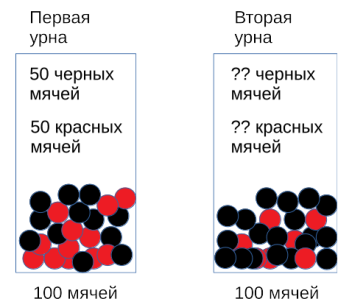
\includegraphics[width=0.5\linewidth]{pictures/pic_expmnt_ellsberg.png}
    \caption{Эксперимент Эллсберга}
    \label{fig:expmnt_ellsberg}
\end{figure}

Более простым примером неопределенности является ситуация связанности независимых событий. Например,
студент плохо готов к экзамену, поэтому ему надо решить, либо идти на экзамен и попытаться
защититься, либо пропустить экзамен и пойти на дополнительную попытку. При этом, студент хочет
полететь на отдых, для чего необходимо купить билеты заренее. Эти два вопроса, о экзамене и покупке
билетов, никак не связаны, однако, студент может быть не удовлетворен результатом экзамена и не полететь
или не сдавать экзамен и спокойно полететь. Иллюстрация этих возможных вариантов событий представлена
на рисунке~\ref{fig:vac_exam}

%\begin{figure}
%    \begin{minipage}[h]{0.4\linewidth}
%        \center{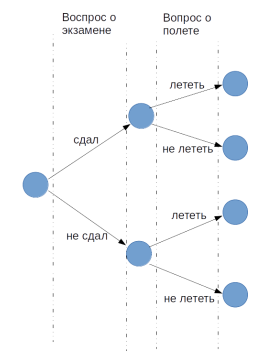
\includegraphics[width=1\linewidth]{pictures/vacation_and_exam.png} \\ а)}
%    \end{minipage}
%    \hfill
%    \begin{minipage}[h]{0.4\linewidth}
%        \center{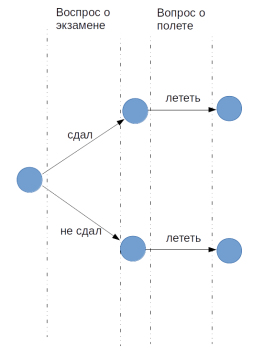
\includegraphics[width=1\linewidth]{pictures/vacation_and_exam_2.png} \\ б)}
%    \end{minipage}
%    \caption{Цепочка событий для двух вопросов a)из эксперимента \citep{shafir199228thinking}, б)по принципу Сэвиджа}
%\end{figure}
\newpage
\begin{figure}[h!]
    \centering
    \captionsetup{justification=centering}
    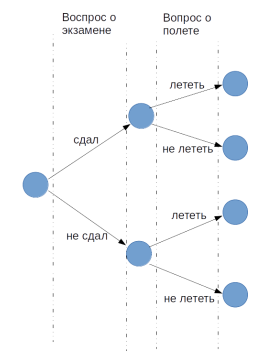
\includegraphics[width=0.35\linewidth]{pictures/vacation_and_exam.png}
    \caption{Цепочка событий для двух вопросов~\citep{shafir199228thinking}}
    \label{fig:vac_exam}
\end{figure}
где кругами обозначаются определенные состояния события. Если использовать принцип уверенности Сэвиджа,
то варианты событий будут выглядеть как на рисунке~\ref{fig:vac_exam_savage}

\begin{figure}[h!]
    \centering
    \captionsetup{justification=centering}
    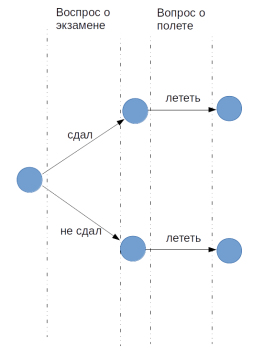
\includegraphics[width=0.35\linewidth]{pictures/vacation_and_exam_2.png}
    \caption{Цепочка событий для двух вопросов по принципу Сэвиджа}
    \label{fig:vac_exam_savage}
\end{figure}
Из этого рисунка видно, что человек всегда выберет один вариант для второго вопроса и при этом ответ
на первый вопрос никак не влияет на второй вопрос. Однако, в этом эксперименте было получено, что
многие люди решили купить билеты в случае провала экзамена или в случае сдачи, но решили не покупать
в случае неизвестных результатов экзамена~\citep{tversky1992disjunction}.

Важным результатом этих экспериментов является выявление эффекта дизъюнкции. Эффект дизъюнкции гласит,
что лучше выбрать вариант $x$ чем $y$, если известно о результате события $S$, или лучше выбрать
вариант $y$ чем $x$, если о результате события $S$ ничего не известно. Данный эффект был сформулирован
в работе Шафира и Тверского~\citep{shafir199228thinking}.

%%%%%%%%%%%%%%%%%%%%%%%%%%%%%%%%%%%%%%%%%%%%%%%%%%%%%%%%%%%%%%%%%%%%%%%%%%%%%%%%%%%%%%%%%%%%%%%%%%%%
%%%%%%%%%%%%%%%%%%%%%%%%%%%%%%%%%%%%%%%%%%%%%%%%%%%%%%%%%%%%%%%%%%%%%%%%%%%%%%%%%%%%%%%%%%%%%%%%%%%%
\section{Роль когнитивных искажений в принятии решений}

Еще один пример с связан ошибкой конъюнкции, который был получен в эксперименте Тверского и
Канемана~\citep{tversky1983extensional}. Эксперимент показывает, что для человека некоторые составные
факты могут быть весомее общих. Для постановки эксперимента, каждому участнику дается информация о
Линде. "Ей 31 год, она одинокая, искренная и очень яркая. Она училась на факультете философии.
Будучи студенткой была обеспокоена вопросами дискриминации и социальной несправедливости, участвовала
в демонстрациях против ядерного оружия". После задавался вопрос: "Какой факт о Линде более вероятен?"
\begin{itemize}
    \item "Линда - кассир в банке";
    \item "Линда - кассир в банке и активная феминистка";
\end{itemize}
Для эксперимента были отобраны 142 студента магистратуры. Для одной половины студентов порядок альтернатив
был прямой, для других обратный, но эта манипуляция не принесла других результатов. В результате 85\%
респондентов выбрали второй вариант: "Линда - кассир в банке и активная феминистка"\citep{tversky2004extensional}.

Эти эффекты показывают, что люди не оценивают все ветви соответствующего дерева решений, даже если
количество результатов велико.

Помимо принятия решения~человеком в условиях неопределенности событий, в когнитивной психологии~рассматриваются
задачи в условиях неопределенности результата решения других людей. Ярким примером такой неопределенности
является дилемма~заключенного. Разница между предыдущими экспериментами заключается в раскрытии большей
информации о неопределенности. Другими словами, респонденту будет известна предположительная информация
о выборе другого человека. Таким образом, предполагается раскрыть больше информации об когнитивных эффектах
происходящих в условиях неопределенности.

Дилемма заключенного является основной задачей теории игр и уже имеет большое количество направлений
исследования. Самым интересным направлением стоит отметить исследования повторяющихся игр, тоесть когда
дилемма заключенного повторяется по неколько раз с теми же игроками. Но не менее интересным стоит
отметить игры на один раз в контексте когнитивной психологии. Разница между многократной и одиночной
игрой заключается в степени неопределенности. Человек абсолютно не знает о другом человеке в первую игру и
не может определить тактику другого человека. При многократном повторении игроки могут угадывать
поведение другого и таким образом неопределеность начинает исчезать.

Но что будет, если игрок будет знать о другом предположительную информацию. В этом случае результат для
первых экспериментов был неожиданным, в них наблюдались эффект неоднозначности и эффект дизъюнкции.
Для объяснения всей сути проблемы необходимо начать с постановки задачи.

В игре учавствуют двое заключенных, каждого из которых поймали во время преступления. Каждому заключенному
дается выбор либо предать друого, либо молчать. Их общий выбор будет влиять на величину наказания для
обоих согласно таблице~\ref{tabular:table_pay}:

\newpage
\begin{table}[h!]
    \caption{Таблица выплат для классической задачи}
    \label{tabular:table_pay}
    \begin{tabular}{cccc}
        "" & "" & \multicolumn{2}{c}{заключенный Б} \\
        "" & "" & молчать & предать \\
        заключенный А &
        \begin{tabular}{r}
            молчать \\
            "" \\
            предать \\
        \end{tabular} &
        \begin{tabular}{|c|}
            \hline
            А - 0.5 года \\
            Б - 0.5 года\\
            \hline
            А - свободен \\
            Б - 10 лет \\
            \hline
        \end{tabular} &
        \begin{tabular}{|c|}
            \hline
            А - 10 лет \\
            Б - свободен \\
            \hline
            А - 2 года \\
            Б - 2 года \\
            \hline
        \end{tabular}
    \end{tabular}
\end{table}
Каждый заключенный знает про эту таблицу и пытается свести результат к минимальному возможному наказанию.
Согласно теории игр, каждому заключенному по Парето-оптимуму необходимо выбирать вариант молчать.
Парето-оптимум позволяет рассматривать задачу для обоих заключенных, позволяет найти общий выйгрыш
для двух заключенных. Рассмотрение задачи для каждого в отдельности позволяет прийти к выводу, что
самым лучшим вариантом является предательство. Поскольку в случае предательства одного заключенного,
промолчавший заключенный получает максимальное наказание. Случай с предательством обоими заключеными
является равновесием Нэша. Согласно равновесию Нэша, существует стратегия или набор стратегий,
изменив которые невозможно получить больший выйгрыш, если друие игроки не поменяли свои стратегии.
Такой стратегией является предательство обоих заключеных, но такая стратегия не является Парето-оптимальным.
Конечно, если заключенные знают друг друга давно и они связаны "воровским законом" или игра является
многократной, то их стратегия оказывается молчание и таким образом равновесие Нэша приближается к
Парето-оптимуму. Но стратегия молчания не работает для других ситуаций, в том числе для однократных
игр, где игроки не знают друг о друге~\citep{kreps1982rational}.

Для экспериментов с людьми удобнее пользоваться другой таблицей выплат, нежели ранее представленной
в таблице~\ref{tabular:table_pay}, которая будет больше интересовать игроков в выйгрыше.
В одной из работ была представлена следующая таблица выплат~\ref{tabular:table_pay_new}.
\begin{table}[h!]
    \caption{Таблица выплат в эксперименте}
    \label{tabular:table_pay_new}
    \begin{tabular}{cccc}
        "" & "" & \multicolumn{2}{c}{игрок Б} \\
        "" & "" & сотрудничать & предать \\
        игрок А &
        \begin{tabular}{l}
            сотрудничать \\
            "" \\
            предать \\
        \end{tabular} &
        \begin{tabular}{|c|}
            \hline
            А - 75 балллов \\
            Б - 75 баллов \\
            \hline
            А - 85 баллов \\
            Б - 25 баллов \\
            \hline
        \end{tabular} &
        \begin{tabular}{|c|}
            \hline
            А - 25 баллов \\
            Б - 85 баллов \\
            \hline
            А - 30 баллов \\
            Б - 30 баллов \\
            \hline
        \end{tabular}
    \end{tabular}
\end{table}
В эксперименте испытуемыми были 80 студентов Принстонского университета. Каждому студенту предоставлялось
по 40 игр из которых 6 были с дилеммой. Другие игры были необходимы для устранения возможности повтора
игроком своей предыдущей стратегии. После прохождения всех игр у каждого участника подсчитывалось количество
баллов, в которые также входили результаты игры с дилеммой (в среднем выплачивалось по 6 долларов).
Игра была разделена на 3 ситуации, где в первой ситуации обыгрывалась стандартная дилемма заключенного,
во второй ситуации игроку предоставлялась информация о сотруднечестве другого игрока, в третьей
ситуации игроку предоставлялась информация о предательстве другого игрока. В результате такой игры
получились результаты представленные в таблице~\ref{tabular:results}
%\begin{wraptable}{r}{0.7\textwidth}
\begin{table}[h!]
    \caption[First caption]{\raggedright Результаты эксперимента дилеммы заключенного}
    \label{tabular:results}
    \begin{tabular}{ccc}
        стандартная игра &
        \begin{tabular}{l}
            предать \\
            сотрудничать
        \end{tabular} &
        \begin{tabular}{c}
            63\% \\
            37\%
        \end{tabular} \\
        \hline
        другой игрок сотрудничает &
        \begin{tabular}{l}
            предать \\
            сотрудничать
        \end{tabular} &
        \begin{tabular}{c}
            84\% \\
            16\%
        \end{tabular} \\
        \hline
        другой игрок предает &
        \begin{tabular}{l}
            предать \\
            сотрудничать
        \end{tabular} &
        \begin{tabular}{c}
            97\% \\
            3\%
        \end{tabular}
    \end{tabular}
\end{table}
%\end{wraptable}

Как видно из этой таблицы, большинство придерживатся стратегии предательства. Также можно заметить, что
некоторые придерживаются стратегии "око за око", в момент когда человек узнает стратегию другого игрока.
Сравнивая результаты стандартной игры и с предоставлением информации игроку, можно заметить, что
большее количество игроков склонно сотрудничать в отсутствие информации о результате выбора другого
игрока (37\%), чем в момент присутствия (16\% и 3\%)~\citep{shafir199228thinking}.
Такое поведение полностью соответствует эффекту дизъюнкции, но можно свести к ошибке конъюнкции, если
принять тот факт, что среднее число вероятности с известным выбором другого (16\% и 3\%) оказывается
меньше вероятности стандартной игры (37\%).

%%%%%%%%%%%%%%%%%%%%%%%%%%%%%%%%%%%%%%%%%%%%%%%%%%%%%%%%%%%%%%%%%%%%%%%%%%%%%%%%%%%%%%%%%%%%%%%%%%%%
%%%%%%%%%%%%%%%%%%%%%%%%%%%%%%%%%%%%%%%%%%%%%%%%%%%%%%%%%%%%%%%%%%%%%%%%%%%%%%%%%%%%%%%%%%%%%%%%%%%%
\section{Значимость парадоксов в принятии решений}

Как~видно из~этого~эксперимента, в~условиях неопределенности испытуемые в стандартной~дилемме~заключенного
более склонны к сотрудничеству, чем в определенных условиях. Все эти эксперименты, перечисленные ранее
представляют основу в данной работе, поскольку с этих работ начинается развитие квантово-подобных моделей.
Стоит отметить, что выводы из экспериментов применимы не только к ситуациям с оппонентом с какой-то
определенной проблемой, но и с другими социальными, экономическими и когнитивными ситуациями. Так например,
проблема дилеммы заключенного применима так же к отношениям между обществом и человеком.

Стоит отметить, что объяcнение всех этих эффектов проводились задолго попыток применения квантового формализма.
Эффект ошибки конъюнкции экспериментаторы Канеман и Тверски пытались объяснить с помощью эвристической
репрезентативности. Однако такой подход является неформальным и плохо определенным, а также учитывают
только ограниченные случаи~\citep{shafffi1990typicality}~\citep{massaro1994pattern}~\citep{gigerenzer1996narrow}.
Существует предположение, что люди склонны оценивать вероятность конъюнкции из некоторой комбинации
вероятностей компонентов, но эмпирических подтверждений этому предположению не существует~\citep{tentori2013determinants}.
Другое предположение основано на понятии индуктивного подтверждения, так же как определено в байесовской
теории, и дают для этого экспериментальное обоснование. Существуют утверждения, что в рамках байесовской
системы существуют случаи когда это не яляется ошибкой и может быть учтена рационально~\citep{von2011bayesian}~\citep{hintikka2004fallacious}.
Конечно, каждый конкретный случай можно смоделировать с помощью простой и логичной модели, но часто
бывают случаи когда модель не применима к другим ситуациям с другими эффектами. В этом случае формализм
квантовой-механики способен соединить различные логические эффекты, которые непосредственно связаны с природой
квантовой механики, в одну или несколько связанных моделей. И таким образом может дать более полное
представление о когнитивных особенностях мышления человека.
    % Глава 2
    %! Author = jaroslav
%! Date = 15.04.20
\chapter{Модели принятия решений в условиях неопределенности}
\section{Открытые квантовые системы}

Это такая система, которая может обмениваться информацией с внешней средой.
В некотором смысле, любая квантовая система является открытой, поскольку на нее могут влиять извне.
Эти воздействия извне создают квантовые шумы, которые мешают рассматривать квантовые системы в простом случае.
Открытые квантовые системы рассматривают ситуацию, когда имеется резервуар и система.
Система может иметь чистое состояние или смешанное и разница состоит в том, что чистое состояние можно
описать как векторами, так и матрицей плотности, а смешанное только матрицей плотности.
Соответственно, динамику для смешанного и для чистого состояния можно задать с помощью следующего уравнения:
\begin{equation}\label{heisenberg}
    \frac{d \rho}{dt} = -i[H,\rho],
\end{equation}
где $H$ - гамильтониан, $\rho$ - матрица плотности.
Но уравнение~\eqref{heisenberg} не описывает динамику с учетом резервуара, поэтому появилось уравнение
Горини-Коссаковского-Сударшана-Линдблада (ГКСЛ):
\begin{equation}
    \frac{d \rho}{dt} = -i[H,\rho] +
    \sum_{j} (C_{j}\rho C^{\dagger}_{j} - \frac{1}{2} C^{\dagger}_{j} C_{j} \rho - \frac{1}{2} \rho C_{j} C^{\dagger}_{j}),
\end{equation}
где $C_{j}$ и $C^{\dagger}_{j}$ - некие операторы анигиляции и рождения, соответственно.
Это уравнение описывает открытые квантовые системы, которые наблюдаются в экспериментах.
Но это уравнение не единственное, которое может описывать открытые квантовые системы, поскольку
квантовые системы могут иметь разные квантовые состояния, которые зависят от резервуара.
А действие резервуара на систему может иметь марковский или немарковский характер.

%%%%%%%%%%%%%%%%%%%%%%%%%%%%%%%%%%%%%%%%%%%%%%%%%%%%%%%%%%%%%%%%%%%%%%%%%%%%%%%%%%%%%%%%%%%%%%%%%%%%
%%%%%%%%%%%%%%%%%%%%%%%%%%%%%%%%%%%%%%%%%%%%%%%%%%%%%%%%%%%%%%%%%%%%%%%%%%%%%%%%%%%%%%%%%%%%%%%%%%%%
\section{Марковские и немарковские системы}

Для рассмотрения немарковских процессов необходимо дать определение марковских процессов.
Марковские процессы — это, в упрощеном понимании, процесс не зависящий от предыдущих состояний системы,
который этот процесс реализует.
Иначе говоря, марковский процесс не имеет памяти и каждое новое состояние, если оно конечно, равновероятно
может произойти в следующий момент времени.
Самыми известными примерами марковских процессов является математическое описание броуновского движения
в газах или~случайное блуждание.
Броуновское движение наблюдается при перемещении микроскопических объектов~в~газах, а случайное блуждание
описывает~математическую~модель случайных изменений в траектории движения точки на плоскости.
Немарковские процессы — это процессы, в упрощенном понимании, зависящие от предыдущих состояний системы.
Самыми известными примерами такого поведения системы можно считать броуновское движение в жидкости,
когда при перемещении микрочастицы жидкость начинает передавать импульс другим частицам и создавать
завихрения, которые могут воздействовать и на частицу.
А так же фликер-шум, который наблюдается в электрических сетях.
Примеры немарковских процессов присутствуют так же и в социальных сетях, так например существует
модель социально значимых интернет-ресурсов.

Помимо этой социальных моделей имеются другие примеры немарковских открытых квантовых систем.
В одном из таких примеров рассматривалось немонотонное изменение параметра расстояния следа
$D(\rho^{1}_{S}, \rho^{1}_{S})$, в случае пары состояний $\rho^{1}_{S}$ и $\rho^{2}_{S}$.
Этот параметр характеризует различимость квантовых состояний.
Суть эксперимента состоит в том, что Алиса передает свои начальные состояния открытой квантовой
системы, связанной с окружающей средой, через зашумленный квантовый канал Бобу.
Из-за взаимодействия среды на канал, этот параметр начинает либо уменьшатся, либо увеличиваться со временем,
что означает либо потерю информации в окружающей среде, либо поступление информации из окружающей среды.
Данный пример схематически показан на рисунке~\ref{fig:state_from_alice_to_bob}.
\begin{figure}[h!]
    \centering
    \captionsetup{justification=centering}
    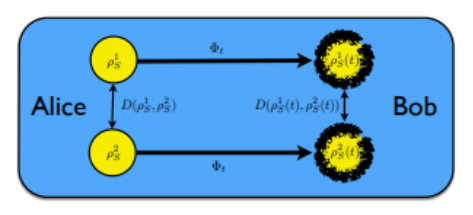
\includegraphics[width=0.7\linewidth]{pictures/state_alice_bob.png}
    \caption{Схема передачи состояния от Алисы к Бобу}
    \label{fig:state_from_alice_to_bob}
\end{figure}
В тот момент, когда система просто теряет информацию, имеет случай марковского процесса, а когда
система получает информацию, имеет случай немарковского процесса.
Получение информации связано с откликом окружающей среды на воздействие открытой квантовой системы,
что свидетельствует о наличии памяти у окружающей среды.

%%%%%%%%%%%%%%%%%%%%%%%%%%%%%%%%%%%%%%%%%%%%%%%%%%%%%%%%%%%%%%%%%%%%%%%%%%%%%%%%%%%%%%%%%%%%%%%%%%%%
%%%%%%%%%%%%%%%%%%%%%%%%%%%%%%%%%%%%%%%%%%%%%%%%%%%%%%%%%%%%%%%%%%%%%%%%%%%%%%%%%%%%%%%%%%%%%%%%%%%%
\section{Дилемма заключенного в квантовом формализме}

Для дилеммы заключенного каждая квантовая модель рассматривается в гильбертовом пространстве, которое
может быть бесконечномерным.
Для системы из двух игроков достаточно конечного пространства.
Определение размерности зависит от количества исходов игры и для этого необходимо определить какие
есть варианты развития событий.
В задаче дилеммы заключенного участвуют двое игроков $G_{1}$ и $G_{2}$ , у каждого из которых есть по два возможных
варианта выбора это сдать и не сдавать, обозначим как вектора в гильбертовом пространстве
$\vert 0 \rangle$ и $\vert 1 \rangle$, соответственно.
Тогда, функцию состояния каждого игрока можно описать с помощью следующей формулы:
\begin{equation}
    \vert \psi \rangle_{j} = \sum_{j=0,1} a_{j} \vert j \rangle
\end{equation}
где $a_{j}$ - коэффициент проекции вектора $\vert j \rangle$.

Такую функцию можно представить с помощью двумерного гильбертова пространства $\mathbb{C}^{2}$.
Квадрат модуля коэффициента $\vert a_{j} \vert^{2}$ имеет смысл как вероятность выбора одного из
векторов $\vert 0 \rangle$ или $\vert 1 \rangle$.
В таком пространстве базисы векторов двух игроков могут быть повернуты на угол друг относительно друга,
а значит в таком случае при выборе одинакового значения двух игроков, направление вектора состояния
будет различаться из-за различного ментального восприятия мира.
При использовании данной формулы можно определить вариант выбора одного игрока, однако на основе
выбора первого невозможно определить выбор другого, иначе говоря их решение не влияет на результат
другого, что в данной дилемме не всегда так, поскольку при повторении игры прошлый опыт влияет на
обоих игроков одновременно.
Поэтому необходимо определить другую функцию состояния, которая впоследствии позволит правильно
определить размерность гильбертова пространства.
Поскольку выбор двух игроков должен влиять друг на друга, то получается они имеют общую функцию
состояния, имеющая следующий вид:
\begin{equation}
    \vert \Psi \rangle_{j} = \sum_{k,l=0,1}^{1} a_{k,l} \vert kl \rangle
\end{equation}
из этой формулы так же видно, что у игроков имеется общее ментальное состояние, что как раз более
правдоподобно в реальном мире.
По аналогии из формулы выше для двумерного гильбертова пространства, $a_{k,l}$ – коэффициент
проекции вектора $\vert kl \rangle$, где $\vert kl \rangle$ – вектор выбора двух игроков
(всего их четыре $\vert kl \rangle$ $\vert kl \rangle$ $\vert kl \rangle$ $\vert kl \rangle$),
а квадрат коэффициента проекции $\vert a_{j} \vert^{2}$ имеет смысл как вероятность выбора исхода игры.

%%%%%%%%%%%%%%%%%%%%%%%%%%%%%%%%%%%%%%%%%%%%%%%%%%%%%%%%%%%%%%%%%%%%%%%%%%%%%%%%%%%%%%%%%%%%%%%%%%%%
%%%%%%%%%%%%%%%%%%%%%%%%%%%%%%%%%%%%%%%%%%%%%%%%%%%%%%%%%%%%%%%%%%%%%%%%%%%%%%%%%%%%%%%%%%%%%%%%%%%%
\section{Модель социально-значимых Интернет ресурсов}

Прежде чем переходить к рассмотрению квантово-подобных моделей принятия решений в условиях неопределенности,
необходимо рассмотреть классические модели, не использующие квантовый формализм. Особенность следующей модели
заключается в том, что ее модель схожа с квантовыми, но не рассматривает остальные социальные задачи, из-за чего
данная модель ограничена в применении.
Это модель социально-значимых Интернет ресурсов, разработанная на основе результатов исследований в социальной
психологии, в механизме запоминания информации человеком, а также на основе теории информации~\citep{pilkevich2015model}.
Данная модель в равной степени адекватно описывает поведение участников сети Интернет ресурсов.

Существует большое количество различных социальных Интернет-ресурсов.
И в первую очередь это различые социальные сети, благодаря которым человек получает персонифицированную информацию
как о себе, так и о других участниках.
Это блоги, благодаря которым человек получает более развернутую информацию.
Различные форумы, которые позволяют обсуждать некоторыую тему и др.
Для предоставления участникам ресурса возможности общения, во многих Интернет-ресурсах требуется предварительная
регистрация.
Определенного шаблона для составления анкеты на этапе регистрации не существует, поскольку различные Интерент-ресурсы
требуют не все данные о пользователе.
Однако, существует некоторая тенденция в составлении анкет во время регистрации, благодаря чему можно спроектировать
модель аккаунта пользователя.

В модели социально-значимых Интернет-ресурсов предлагается модель пользовательского аккаунта.
Эта модель описывает большое количество различных параметров анкеты пользователя.
Эта модель имеет следующий вид:
\begin{equation}
    A = <Pers, Cont, CoC, Prof>,
\end{equation}
где $Pers$ — подмножество идентифицирующей информации, $Cont$ — подмножество контактных данных,
$CoC$ — подмножество данных о социальных связях, $Prof$ — подмножество различной личной информации.

Помимо этого, для этой модели существует модель распространения информации, которая имеет вид:
\begin{equation}
    I = <Pers, M, T>,
\end{equation}
где $Pers$ — подмножество идентифицирующей информации, $M$ — мнения, комментарии,
$T$ — отметка времени, $K = f(M)$ — когниция, элемент знания (данные, усвоенные сознанием).

Помимо этого, модель пользовательского аккаунта имеет информацию о связях с другими аккаунтами,
которая позволяет рассчитать параметр интенсивности отношений:
\begin{equation}\label{alphaik}
    \alpha_{ik} = N log_{2} \frac{N_{ik}}{N_{0}},
\end{equation}
где $N_{ik}$ – количество переданых сообщений/знаков между членами $i$ и $k$,
$N_{0}$ – среднее значение переданных сообщений в сообществе, $N$ – некоторая константа, различная для каждого индивида.

На основе формулы \ref{alphaik}, а также модели пользовательского аккаунта и модели распространения информации
приводится схема взаимодействия пользователей и информации в виде графа (см. рисунок \ref{fig:shema_system_in_socium}).

\begin{figure}[h!]
    \centering
    \captionsetup{justification=centering}
    \includegraphics[width=0.8\linewidth]{pictures/shema_system_in_socium.png}
    \caption{Схема системы психологических отношений в социуме (социально значимых Интернет-ресурсах)}
    \label{fig:shema_system_in_socium}
\end{figure}

На этом рисунке $A = \{ A_{1}, A_{2}, A_{3}, \dots, A_{N}\}$ – это члены сети,
$K = \{ K_{1}, K_{2}, K_{3}, \dots, K_{N}\}$ – это когниции.~Схема построена с учетом теории когнитивного
~диссонанса Л.~Фестингера,~теории структурного баланса Ф.~Хайдера, теории коммуникационных актов Т.~Ньюкома
и теории конгруэнтности Ч.~Осгуда и П.~Танненбаума, для которых базовыми постулатами являются предположения
о возможности получения человеком информации, его переработке, его усвоению, о стремлении человека к наибольшей
связности имеющихся знаний, которые могут побуждать к действиям.

Самым~простым элементом отношений в этой схеме является рассмотрение двух членов социума (O,S) и одной когниции (K).
Смена значений этих отношений называется как информационно-психологическая акция (ИПА).
Данная ИПА представлена на Рисунке~\ref{fig:shema_OSK}.
\begin{figure}[h!]
    \centering
    \captionsetup{justification=centering}
    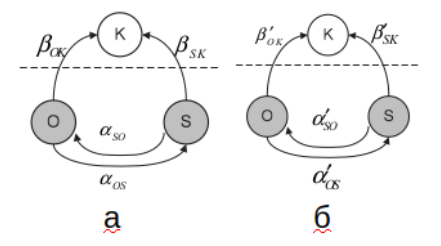
\includegraphics[width=0.7\linewidth]{pictures/schema_OSK.png}
    \caption{Схема отношений объекта O и субъекта S друг к другу и к утверждению K: a)
    для события до ИПА; б) после ИПА~\citep{pilkevich2015model}}
    \label{fig:shema_OSK}
\end{figure}
На рисунке~\ref{fig:shema_OSK}~а параметры $\alpha_{OS}, \alpha_{SO}$ показывают отношение объекта и субъекта
друг к другу, параметры $\beta_{OK}, \beta_{SK}$ показывают отношение членов социума к утверждению.
На рисунке~\ref{fig:shema_OSK}~б, эти отношения имеют новые значения и обозначаются
$\alpha^{\prime}_{OS}, \alpha^{\prime}_{SO}, \beta^{\prime}_{OK}, \beta^{\prime}_{SK}$
Изменение значений для параметров отношений вычисляются на основе дифференциалов Осгуда и для этой модели
записываются следующим образом:
\begin{equation}
    \Delta_{OK} = \frac{|\alpha_{OS}|}{|\beta_{OK}|+|\alpha_{OS}|} |\beta_{OK}-\alpha_{OS}|,\\
    \Delta_{OS} = \frac{|\beta_{OK}|}{|\beta_{OK}|+|\alpha_{OS}|} |\beta_{OK}-\alpha_{OS}|
\end{equation}
где $\Delta_{OK}, \Delta_{OS}$ – это приращение к $\beta_{OK}, \alpha_{OS}$ соответственно.
Различные ситуации взаимоотношений между элементами {O,S,K} были рассмотрены в теории структурного
баланса Ф.~Хайдера, а изменение отношений рассмотрено в теории коммуниуативных актов Т.~Ньюкомба,
благодаря чему известны формулы для $\beta^{\prime}_{OK}, \alpha^{\prime}_{OS}$, которые получаются
от начальных параметров отношений $\beta_{OK}, \alpha_{OS}$ и приращений к ним $\Delta_{OK}, \Delta_{OS}$.

В работах по моделированию информационно-психологических отношений наблюдается явление, при котором
элемент социума при получения некоторой когниции распространяет его вторично.
Формула, по которой это вторичное распространение информации описывется имеет вид:
\begin{equation}\label{beta_ij}
    \beta_{ij}(t) = \beta_{ij}(t_0)\cos(\rho_{i}\sqrt{t-t_0})e^{-\lambda_{i}(t-t_0)},
\end{equation}
где $t_0$ – время последнего изменения отношения элемента социума к когниции (утверждению), $t$ – текущее
время изменения, $\lambda_{i}$ – коэффициент «старения и утраты уникальности утверждения», $\rho_{i}$ –
коэффициент когнитивного «резонанса», вторичного распространения информации.
График данной функции представлен на рисунке~\ref{fig:graphic_beta}
\begin{figure}[h!]
    \captionsetup{justification=centering}
    \begin{minipage}[h]{0.4\linewidth}
        \center{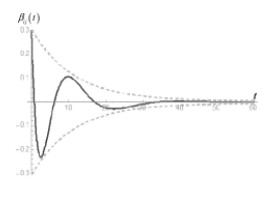
\includegraphics[width=1\linewidth]{pictures/graphic_beta_a.png} \\ а)}
    \end{minipage}
    \hfill
    \begin{minipage}[h]{0.4\linewidth}
        \center{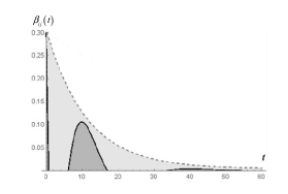
\includegraphics[width=1\linewidth]{pictures/graphic_beta_b.png} \\ б)}
    \end{minipage}
    \caption{Уровень отношения $\beta_{ij}(t)$ члена сети $A_{i}$ к утверждению $K_{j}$~\citep{pilkevich2015model}}
    \label{fig:graphic_beta}
\end{figure}

Данный график, к сожалению, не показывает других зависимостей этой функции от других параметров, но
на нем хорошо видно как ведет функция себя при постоянных параметрах.
На рисунке~\ref{fig:graphic_beta}а показан полный вариант с положитеьлными и отрицательными полупериодами.
Отрицательные полупериоды показывают маловероятное проявление когнитивной активности.
Положительные полупериоды показывает наиболее вероятное проявление когнитивной активности.
Для более детального рассмотрения графика функции $\beta_{ij}(t)$, на рисунке~\ref{fig:beta_another_param}
представлены зависимости с дополнительным параметром ($\lambda_{i}$).
\begin{figure}[h!]
    \centering
    \captionsetup{justification=centering}
    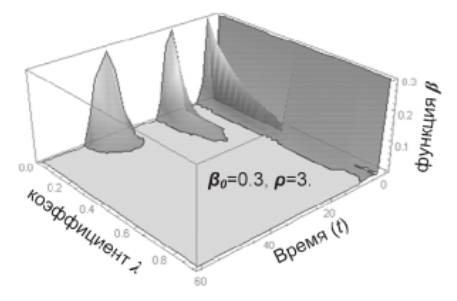
\includegraphics[width=0.7\linewidth]{pictures/graphic_beta_anotherparam.png}
    \caption{График функции $\beta_{ij}(t)$ с динамикой параметра $\lambda_{i}$~\citep{pilkevich2015model}}
    \label{fig:beta_another_param}
\end{figure}

Как видно из этого и предыдущего графиков, что существуют семейства монотонно убывающих зависимостей
Эббингауза при определенных значениях параметра $\lambda_{i}$.
Однако, как подчеркнули сами авторы, данную модель невозможно использовать в практической деятельности,
но предлагают ограничение этой модели в определенных коэффициентах для определенных однородных групп,
иначе говоря групп состоящих из людей с одним уровнем образования или предпочтений.
Таким образом диапазон модели для $4.5 < \rho_{i} < 5$ представлен на рисунке~\ref{fig:beta_4_5rho5}
\newpage
\begin{figure}[h!]
    \centering
    \captionsetup{justification=centering}
    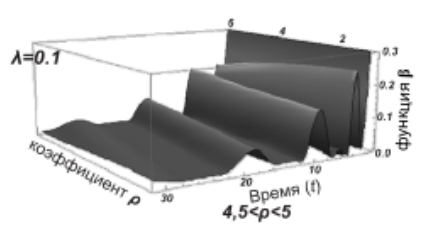
\includegraphics[width=0.7\linewidth]{pictures/graphic_beta_45rho5.png}
    \caption{График функции $\beta_{ij}(t)$ с динамикой параметра $\rho_{i}$~\citep{pilkevich2015model}}
    \label{fig:beta_4_5rho5}
\end{figure}

В работе утверждается, что данное поведение похоже на социальную диффузию, которое представляется как
\glqqкогнитивный шум\grqq.
Интересно также то, что данный шум показывает момент перехода мнения человека к мнению группы, что так
же подтверждает справедливость уменьшения диапазонов $\rho_{i}$ и $\lambda_{i}$.

Теперь рассмотрим эту проблему с точки зрения известных квантово-подобных моделей.
%\section{Пояснение связей экспериментов и модели}
%Связь между моделью социално-значимых Интернет ресурсов и когнитивными экспериментами заключается в
%вывляении общих рассматриваемых объектов.
%Такими объектами в экспериментах является человек или два человека и некоторый вопрос или утверждение,
%а в модели имеются два человека и утверждение.
%Это значит, что множество объектов для экспериментов и для модели имеет одну и ту же структуру.
%Схема этой структуры представлена на рисунке~\ref{fig:chain_struct}
%\begin{figure}[h!]
%    \centering
%    \captionsetup{justification=centering}
%    \includegraphics[width=0.5\linewidth]{pictures/chain_struct.png}
%    \caption{Человек и утверждение}
%    \label{fig:chain_struct}
%\end{figure}
%
%В~данном~случае~человек (агент) находится внутри~этой когниции (утверждения), таким образом агент
%воспринимает когницию как окружающий мир.
%Взаимодействие между агентом и когницией подчинятеся модели социально-значимых ресурсов~\eqref{beta_ij}.
%Причина, по которой не указано два агента, заключается в отсутствии влияния другого агента на когницию.
%Влияние агента на когницию не происходит, а происходит изменение только отношения агента к когниции.
%Это легко заметить в окружающем мире, факты о каком-либо событии невозможно изменить, их можно только
%поменять или не указывать.

%    % Глава 3
    %! Author = jaroslav
%! Date = 17.04.20
\chapter{Глава третья}
\section{Часть третья}

Ранее был рассмотрен эксперимент с дилеммой заключенного и его сформулированный эффект.
Этот эффект хорошо моделируется с помощью квантово-подобных моделей принятия решений, благодаря
тому, что неопределенность описывется квантовой суперпозицией с точки зрения одного из игроков.
Таким образом описание неопределенности для игрока А относительно игрока Б описывается следующим образом:
\begin{equation}\label{phi_B}
    \vert \phi_{B} \rangle = \alpha \vert 0_{B} \rangle + \beta \vert 1_{B} \rangle \in \mathbb{C}^{2} % \mathbf{C}^{2}
\end{equation}
где $\alpha$ и $\beta$ - показывают степень осознания действия игрока Б, $\vert 0_{B} \rangle$ - характеризует
вектор предательства игроком Б, $\vert 1_{B} \rangle$ - характеризует вектор сотрудничества игроком Б.
$\mathbb{C}^{2}$ - двумерное комплексное пространство (в данном случае Гильбертово).
Для описания ситуации с учетом принятия решения игрока А, необходимо использовать четырехмерное Гильбертово
пространство $\mathbb{C}^{2} \otimes \mathbb{C}^{2}$.
В таком случае уравнение \eqref{phi_B} имеет следующий вид, в случае предательства игрока А~\citep{asano2011quantum}:
\begin{equation}
    \vert \Phi_{0_{A}} \rangle = \alpha_{0} \vert 0_{A} 0_{B} \rangle + \beta_{0} \vert 0_{A} 1_{B} \rangle \in \mathbb{C}^{2} \otimes \mathbb{C}^{2}
\end{equation}
С учетом сотрудничества игрока А, вектор общего психического состояния системы двух игроков записывается
следующим образом:
\begin{equation}
    \vert \Psi \rangle = \sum_{x,y=0}^{1} \alpha_{x,y} \vert x_{A} y_{B} \rangle =
    \alpha_{0} \vert 0_{A} 0_{B} \rangle + \beta_{0} \vert 0_{A} 1_{B} \rangle +
    \alpha_{1} \vert 1_{A} 0_{B} \rangle + \beta_{1} \vert 1_{A} 1_{B} \rangle
\end{equation}

Этот подход для описания состояния двух игроков позволяет рассматривать проблему на коллективном уровне.
Так например можно применить теорию открытых квантовых систем и рассматривать игрока А как квантовую
систему, а игрока Б как резервуар~\citep{bagarello2015operator,bagarello2015quantum}.
В этом случае игрока А будем обозначать как Алиса или агент $a$, а игрока Б как резервуар $b$.
В квантовой теории поля применима процедура квантования, основанная на алгебре операторов рождения
и уничтожения $a, a^{\dagger}, b, b^{\dagger}$.
Эти операторы позволяют рассматривать переход из одного квантового состояния в другое.
\begin{equation}
    \vert 1_{A} 0_{B} \rangle = a^{\dagger} \vert 0_{A} 0_{B} \rangle,
    \vert 0_{A} 1_{B} \rangle = a b^{\dagger} \vert 1_{A} 0_{B} \rangle
\end{equation}
Для данных операторов действуют следующие коммутационные соотношения:
\begin{equation}\label{CCR}
    [ a, a^{\dagger} ] = 1,
    [ b(k), b^{\dagger}(k) ] = \delta (k-k')
\end{equation}
где $k$ - размернность резервуара, $[x,y] = xy - yx$ - коммутатор.
Зная коммутационное соотношение~\eqref{CCR}, можно определить числовой оператор $n_a=a^{\dagger}a$
для агента.
Собственное значение этого оператора соответствует выбору, которым оперирует агент~\citep{bagarello2015quantum}.
Для определения операторов агента и резервуара используется уравнение Гейзенберга, которое имеет вид:
\begin{equation}
    i \hbar \frac{\partial f}{\partial t} = [f, H]
\end{equation}
где $i$ - мнимая единица, $\hbar$ - постоянная Планка, $\frac{\partial f}{\partial t}$ - дифференциал
функции $f$ по времени $t$, $[\cdot, \cdot]$ - коммутатор, $H$ - гамильтониан.
Для решения этого уравнения необходимо знать гамильтониан, который имеет вид:
\begin{multline}
    H = H_f + H_R + H_{int} = \hbar \omega_a a^{\dagger} a + \hbar \int \omega_{R}(k) b^{\dagger}(k) b(k) d^{D}(k) \\
    + \hbar \lambda \int g(k)(b^{\dagger}(k) a + a^{\dagger} b(k)) d^{D}(k)
\end{multline}
где $H_f$ - гамильтониан описывающий агента, $H_R$ - гамильтониан описывающий резервуар, $H_{int}$ -
гамильтониан взаимодействия резервуара и агента, $\omega_{a}$ - частотная характеристика агента,
$\omega_{R}(k)$ - частотная характеристика резервуара, $g(k)$ - параметр плотности резервуара,
$\lambda$ - коэффициент взаимодействия резервуара и агента.
В результате решения этого уравнения для операторов получаем систему уравнений:
\begin{equation}
    \begin{cases}
        & \dot{a}(t) = -i \omega_a a(t) - i \lambda \int g(k)b(k,t) d^{D}(k) \\
        & \dot{b}(k,t) = -i \omega_{R}(k) b(k,t) -i \lambda g(k)a(t)
    \end{cases}
\end{equation}
Решение дифференциального уравнения для динамики оператора $\dot{b}(k,t)$ с начальными условиями
$b(k,0)=b(k)$ имеет следующий вид:
\begin{equation}
    b(k,t) = b(k)e^{-i \omega_{R}(k) t}-i \lambda \int_{0}^{t} g(k)a(\tau)e^{-i \omega_{R}(k) (t-\tau)} d\tau
\end{equation}
В результате полученного решения для $b(k,t)$, дифференциальное уравнение для $a(t)$ имеет следующий вид:
\begin{multline}\label{dotat_bagarello}
    \dot{a}(t) =
    -i \omega_{a} a(t)
    -i \lambda \int g(k)b(k)e^{-i \omega_{R}(k) t} d^{D}(k) \\
    -\lambda^{2} \iint_{0}^{t} g^{2}(k) a(\tau) e^{-i \omega_{R}(k) (t-\tau)} d\tau d^{D}(k)
\end{multline}
Решение этого уравнения является нетривиальной задачей, поскольку двойной интеграл в третьем слагаемом
никак не сокращается.
Частным решением этого уравнения является принятие постоянных значений переменных $g(k) = 1$ и
$\omega_{R}(k) = \omega_{b} k$~\citep{bagarello2018quantum}.
Благодаря чему уравнение~\eqref{dotat_bagarello} имеет следующий вид:
\begin{equation}
    \dot{a}(t) =
    - \Biggl(i \omega_{a} + \frac{\pi \lambda^{2}}{\omega_{b}} \Biggr) a(t)
    -i \lambda \int b(k)e^{-i \omega_{b} k t} d^{D}(k)
\end{equation}
Такое уравнение достаточно просто решается и его решение имеет вид:
\begin{equation}\label{at_bagarello}
    a(t) = \Biggl( a - i \lambda \int b(k) \eta(k,t) d^{D}(k) \Biggr)
    e^{-\bigl(i \omega_{a} + \frac{\pi \lambda^{2}}{\omega_{b}} \bigr) t}
\end{equation}
где $\eta(k,t) = \frac{1}{\rho(k)}(e^{\rho(k) t} - 1)$,
$\rho(k) = i\omega - i\omega_{b} k + \frac{\pi \lambda^{2}}{\omega_{b}}$~\citep{bagarello2018quantum}.
Уравнение~\eqref{at_bagarello} подчиняется правилу коммутации.
Зная свойство для операторов резервуара $\langle b^{\dagger}(k) b^{k'} \rangle = n_{b} \delta (k-k')$,
а также свойство для динамики числового оператора $n_{a}(t) = a^{\dagger}(t) a(t)$, который в последующем
будем просто называть оператор принятия решения, можем получить решение числового оператора агента:
\begin{equation}\label{na_bagarello}
    n_{a}(t) = n_{a} e^{- \frac{2 \lambda \pi}{\omega_{b}} t} + n_{b} \Biggl( 1 - e^{\frac{2 \lambda \pi}{\omega_{b}} t} \Biggr)
\end{equation}
Эта модель при $ t \rightarrow \infty$ стремится к фиксированному значению $n_{b}$, что как раз
представлено на рисуке~\ref{fig:at_baga}
\begin{figure}[h!]
    \captionsetup{justification=centering}
    \begin{minipage}[h]{0.49\linewidth}
        \center{\includegraphics[width=1\linewidth]{pictures/at_baga_0.png} \\ а)} \\
    \end{minipage}
    \begin{minipage}[h]{0.49\linewidth}
        \center{\includegraphics[width=1\linewidth]{pictures/at_baga_01.png} \\ б)}
    \end{minipage}
    \begin{minipage}[h]{0.49\linewidth}
        \center{\includegraphics[width=1\linewidth]{pictures/at_baga_05.png} \\ в)} \\
    \end{minipage}
    \begin{minipage}[h]{0.49\linewidth}
        \center{\includegraphics[width=1\linewidth]{pictures/at_baga_1.png} \\ г)}
    \end{minipage}
    \caption{Характер поведения модели при $n_{b}$ равном: а)0; б)0,1; в)0,5; г)1}
    \label{fig:at_baga}
\end{figure}

Как видно из этого рисунка, характер поведения модели схож по поведению модели социально-значимых
Интернет ресурсов при параметре $\rho_{i} = 1$.
Однако, в данной модели не рассматриваются другие частные случаи для параметров $g(k)$ и $\omega_{R}(k)$.

%%%%%%%%%%%%%%%%%%%%%%%%%%%%%%%%%%%%%%%%%%%%%%%%%%%%%%%%%%%%%%%%%%%%%%%%%%%%%%%%%%%%%%%%%%%%%%%%%%%%
%%%%%%%%%%%%%%%%%%%%%%%%%%%%%%%%%%%%%%%%%%%%%%%%%%%%%%%%%%%%%%%%%%%%%%%%%%%%%%%%%%%%%%%%%%%%%%%%%%%%
\section{Часть четвертая}

В этой части рассматривается $\omega_{R}(k) = \omega k$, а параметр плотности $g(k)$ подчиняется
следующему уравнению:
\begin{equation}\label{gk}
    g^{2}(k) = \frac{g}{k^{2} + \alpha^{2}},
\end{equation}
Подставляя уравнение~\eqref{gk} в уравнение~\eqref{dotat_bagarello} и приняв во внимание тот факт, что
\begin{equation}
    \int \frac{e^{-i \omega k (t - \tau)}}{k^{2} + \alpha^{2}} dk = \frac{\pi}{\alpha} e^{-\alpha \omega (t - \tau)}
\end{equation}
получаем новый вид оператора $\dot{a}(t)$:
\begin{equation}\label{dotat}
    \dot{a}(t) =
    -i \omega_{a} a(t)
    -i \lambda \sqrt{g} \int \frac{b(k)e^{-i \omega k t}}{\sqrt{k^{2} + \alpha^2}} dk
    -\frac{\lambda^{2} g \pi}{\alpha} \int_{0}^{t} a(\tau) e^{- \alpha \omega (t - \tau)} d\tau
\end{equation}
Решать данное уравнение стандартно не получится, поскольку третье слагаемое невозможно вывести из
под знака интеграла.
В данной работе будет использоваться два способа решения этой задачи.
Первый способ будет заключаться в поиске непосредственно оператора принятия решения $n_{a}$ числовым
методом, не получая вид оператора агента $a^{\dagger}(a)$.
Второй способ заключается в поиске оператора рождения(уничтожения) для агента $a^{\dagger}(a)$ числовым
методом, а после числовым методом определить оператор принятия решения $n_{a}$.

%%%%%%%%%%%%%%%%%%%%%%%%%%%%%%%%%%%%%%%%%%%%%%%%%%%%%%%%%%%%%%%%%%%%%%%%%%%%%%%%%%%%%%%%%%%%%%%%%%%%
%%%%%%%%%%%%%%%%%%%%%%%%%%%%%%%%%%%%%%%%%%%%%%%%%%%%%%%%%%%%%%%%%%%%%%%%%%%%%%%%%%%%%%%%%%%%%%%%%%%%
\section{Первый способ моделирования}

Зная свойство оператора принятия решения $n_{a}(t) = a^{\dagger}(t) a(t)$, а также правило
дифференцирования $(xy)' = x'y + xy'$, можно получить итерационное числовое решение этой модели:
\begin{multline}
    n_{a}(t + \Delta t) =
    \Biggl[i \lambda \sqrt{g} \int \frac{R_{1}(k,t) e^{i \omega k t} - R_{2}(k,t) e^{-i \omega k t}}{\sqrt{k^{2} + \alpha^2}} dk - \\
    - 2 \frac{\lambda^{2} g \pi}{\alpha} n_{a}(t) \Biggr] \Delta t + n_{a}(t)
\end{multline}
\begin{multline}
    R_{1}(k,t + \Delta t) =
    \Biggl[-i \omega_{a} R_{1}(k,t)
    -i \lambda \sqrt{g} \frac{n_{b} e^{-i \omega k t}}{\sqrt{k^{2} + \alpha^2}} - \\
    -\frac{\lambda^{2} g \pi}{\alpha} \int_{0}^{t} R_{1}(k,\tau) e^{- \alpha \omega (t - \tau)} d\tau \Biggr] \Delta t + R_{1}(k,t)
\end{multline}
\begin{multline}
    R_{2}(k,t + \Delta t) =
    \Biggl[i \omega_{a} R_{2}(k,t)
    + i \lambda \sqrt{g} \frac{n_{b} e^{i \omega k t}}{\sqrt{k^{2} + \alpha^2}} + \\
    - \frac{\lambda^{2} g \pi}{\alpha} \int_{0}^{t} R_{2}(k,\tau) e^{- \alpha \omega (t - \tau)} d\tau \Biggr] \Delta t + R_{2}(k,t)
\end{multline}
Все стадии получения этих уравнений приедены в приложении.
Остается вопрос с параметрами для модели, какие они должны быть и подчиняются ли они какому-либо закону.
Правило по которому параметры не могут иметь случайные величины основано на коммутационном соотношении
для динамки операторов агента:
\begin{equation}\label{dynamic_comm-1}
    [\dot{a}(t),\dot{a}^{\dagger}(t')] = \frac{\partial}{\partial t} \frac{\partial}{\partial t'} \delta (t-t') =
    \dot{a}(t) \dot{a}^{\dagger}(t') - \dot{a}^{\dagger}(t') \dot{a}(t) = 0
\end{equation}
Это коммутационное соотношение имеет другой вид:
\begin{equation}\label{dynamic_comm}
    [\dot{a}(t),\dot{a}^{\dagger}(t')] = \omega^{2}_{a} + \lambda^{2} g \frac{\pi}{\alpha} +
    \frac{\lambda^{4} g^{2} \pi^{2}}{2 \alpha^{3} \omega} (1-e^{-2 \alpha \omega t}) = 0
\end{equation}
Все стадии вычислений смотреть в приложении.
Это уравнение можно переписать в другом виде:
\begin{equation}
    g_{1,2} = \frac{\omega \alpha^{2}}{\lambda^{2} \pi (1-e^{-2 \alpha \omega t})}
    \Biggl( -1 \pm \sqrt{1 - 2 \frac{\omega^{2}_{a} }{\alpha \omega} (1-e^{-2 \alpha \omega t})} \Biggr)
\end{equation}
В дальнейшем разница между $g_{1}$ и $g_{2}$ не будет играть большой роли, поскольку это никак не будет
влиять на окончательный результат модели.

Стоит отметить, что $g \in \mathbb{R}$ и $g > 0$, связано это с тем, что параметр $g$ в уравнении~\eqref{dotat}
заключен под корнем и отрицательное значение $g$ приведет к комплексному значению параметра принятия решения.
Параметр принятия решения $n_a$ должен быть $n_a \in \mathbb{R}$.

%%%%%%%%%%%%%%%%%%%%%%%%%%%%%%%%%%%%%%%%%%%%%%%%%%%%%%%%%%%%%%%%%%%%%%%%%%%%%%%%%%%%%%%%%%%%%%%%%%%%
%%%%%%%%%%%%%%%%%%%%%%%%%%%%%%%%%%%%%%%%%%%%%%%%%%%%%%%%%%%%%%%%%%%%%%%%%%%%%%%%%%%%%%%%%%%%%%%%%%%%
\section{Граничные условия параметра плотности}

Параметр $g$ имеет два решения:
\begin{equation}\label{gplus}
    g_{1} = \frac{\omega \alpha^{2}}{\lambda^{2} \pi (1-e^{-2 \alpha \omega t})}
    \Biggl( -1 + \sqrt{1 - 2 \frac{\omega^{2}_{a} }{\alpha \omega} (1-e^{-2 \alpha \omega t})} \Biggr),
\end{equation}
\begin{equation}\label{gminus}
    g_{2} = \frac{\omega \alpha^{2}}{\lambda^{2} \pi (1-e^{-2 \alpha \omega t})}
    \Biggl( -1 - \sqrt{1 - 2 \frac{\omega^{2}_{a} }{\alpha \omega} (1-e^{-2 \alpha \omega t})} \Biggr),
\end{equation}
Ранее для этого параметра было обнаружено, что его значение не должно быть комплексным или отрицательным,
поскольку этом случае для уравнения $n_{a}$ решения не существует.
Иначе говоря, оператор принятия решения $n_{a}$ становится комлексным числом.
Рассмотрим первое уравнение для параметра~\eqref{gplus}.
Это уравнение имеет решение, если $\alpha, \omega, \lambda, t \neq 0$.
Видно, что в начальный момент времени $t = 0$ это уравнение не применимо, однако этого не требуется
по решению основного уравнения, поскольку в начальный момент времени необходимые параметры уже заданы.
\begin{equation}\label{first_frac}
    \frac{\omega \alpha^{2}}{\lambda^{2} \pi (1-e^{-2 \alpha \omega t})},
\end{equation}
Первая дробь~\eqref{first_frac} имеет отрицательное значение при $\alpha < 0$.
В данном уравнении $\omega$ и $t$ не может быть отрицательным, поскольку время отсчитывается от
момента наблюдения, а отрицательной частоты быть не может.
Поэтому на знак вляет только два параметра.
Теперь рассмотрим в уравнении~\eqref{gplus} выражение под корнем:
\begin{equation}\label{last_square}
    \sqrt{1 - 2 \frac{\omega^{2}_{a} }{\alpha \omega} (1-e^{-2 \alpha \omega t})}
\end{equation}
Выражение~\eqref{last_square} должно быть строго положительное.
Теперь предположим, что $\alpha < 0, \omega > 0$.
В таком случае уравнение~\eqref{last_square} можем переписать в следующем виде:
\begin{equation}\label{last_square_two}
    \sqrt{1 + 2 \frac{\omega^{2}_{a} }{\vert \alpha \vert \omega} (1-e^{2 \vert \alpha \vert \omega t})}
\end{equation}
С~увеличением~времени~экспонента~начинает~возрастать,~а это значит, выражение в скобках будет~отрицательное~
$(1~-~e^{2 \vert \alpha \vert \omega t})~<~0$.
Раз оно отрицательное, значит второе слагаемое~под корнем будет так же отрицательное в выражении~\eqref{last_square_two}.
Поскольку все переменные в выражениях~\eqref{last_square} и~\eqref{last_square_two} являются
действительными числами, то на знак под корнем может зависеть только от $\alpha$.
Значит, второе слагаемое в выражениях~\eqref{last_square} и~\eqref{last_square_two} всегда будет отрицательное.

В таком случае рассмотрим следующее неравенство:
\begin{equation}
    2 \frac{\omega^{2}_{a} }{\alpha \omega} (1-e^{-2 \alpha \omega t}) < 1
\end{equation}
Если рассмотреть предел по $ t \rightarrow \infty$, то левая часть неравенства стремится к бесконечности.
Изменением переменных $\alpha$ и $\omega$, неравенство не соблюдается, покольку при увеличении этих
переменных, увеличивается и степень в экспоненте.
Значит необходимо определить границы переменной $\omega_{a}$, которые приведены в выражении~\eqref{omega_a}:
\begin{equation}\label{omega_a}
    \omega^{2}_{a} < \frac{\alpha \omega}{2(1-e^{2 \alpha \omega t})}
\end{equation}
Рассмотрим правую часть неравенства в пределе $t \rightarrow \infty$.
Пусть в этом случае $\alpha > 0$, тогда в пределе неравенство имеет следующий вид:
\begin{equation}\label{omega_a_2}
    \omega^{2}_{a} < \frac{\alpha \omega}{2}
\end{equation}
в случае $\alpha < 0$:
\begin{equation}\label{omega_a_3}
    \omega^{2}_{a} < \frac{\alpha \omega}{\infty} \rightarrow \omega^{2}_{a} = 0
\end{equation}
причина, по которой неравенство превратилось в равенство для $\omega_{a}$, заключается в неосуществимости
отричательной частоты.
Случай выражения~\eqref{omega_a_2} легко соблюдать, однако если решать уравнение~\eqref{gplus} с
параметром $\alpha > 0$, то зачение выражения~\eqref{gplus} будет $g < 0$, что не допустимо.
Значит нужно рассматривать случай для выражения~\eqref{omega_a_3}, поскольку только в этом случае $g > 0$.
Такие же значения выражения~\eqref{gplus} при данных параметрах, справедливы для выражения~\eqref{gminus}.
Из этого заключаем вывод, что значения должны быть следующие: $\omega^{2}_{a} = 0, \alpha < 0$.

Если внимательно рассмотреть результаты ограничений, то можно заметить отсутствие частотной характеристики
агента $\omega^{2}_{a} = 0$, чего не может происходить в рассматриваемой модели, поскольку это означает
отсутвие самого агента в резервуаре.
Отсутвие агента в резервуаре делает бессмысленным дальнейшее моделирование.
Было выдвинуто предположение, что была совершена ошибка во время вычисления и для выявления ошибки
необходимо проверить величины для каждого параметра: $k$ - безразмерный, $\lambda$ - безразмерный,
$g(k)$ - [Гц], $\omega$ - [Гц], $\omega_{a}$ - [Гц], $\alpha$ - безразмерный.
В результате было обнаружено, что в коммутаторе~\eqref{dynamic_comm} не совпадают размерности при вычислении.
Для чего была сделана нормировка значений по $g$ начиная с уравнений гамильтонианов, результаты которых
приведены в приложении.
Однако такой способ исключения ошибки не дал результатов в уравнении~\eqref{dynamic_comm}, поэтому
вопрос об ошибке в вычислениях остается открытым.
Возможно ошибка случается из-за того, что дельта-функция Дирака является не дифференцируемой функцией,
а значит и коммутатор~\eqref{dynamic_comm-1} нельзя приравнять к нулю.

%%%%%%%%%%%%%%%%%%%%%%%%%%%%%%%%%%%%%%%%%%%%%%%%%%%%%%%%%%%%%%%%%%%%%%%%%%%%%%%%%%%%%%%%%%%%%%%%%%%%
%%%%%%%%%%%%%%%%%%%%%%%%%%%%%%%%%%%%%%%%%%%%%%%%%%%%%%%%%%%%%%%%%%%%%%%%%%%%%%%%%%%%%%%%%%%%%%%%%%%%
\section{Результаты вычисления первым способом}

Даже несмотря на присутствие комплексной составляющей в результатах вычислений, получить результат
схожий с марковскими квантово-подобными моделями оказалось невозможным для первого способа.
Также, не удалось получить подобие модели~социально-значимых Интернет ресурсов, но результаты и их
объяснение стоит привести для понимания проблемы моделирования.
Прежде всего стоит начать с тех результатов полученной модели, при котором наблюдается осцилляции в
поведении модели.
Разработанная модель подразумевает осцилляции при любых параметрах, и таким образом они будут присутствовать
всегда, разница будет заключаться в том насколько сильно они будут влиять на конечный результат.
Влияние на конечный результат может наблюдаться совершенно по разному и при порой неожиданных результатах.
У модели, разработанной данным способом, очень сложно предсказывается поведение как раз по причине
дополнительной комплексной составляющей, который дает параметр $g$.
Так например на рисунке~\ref{fig:fr_oscillation} осилляции очень быстро выводят агента из состояния
равновесия, причем характер осцилляций даже усиливается.
\begin{figure}[h!]
    \centering
    \captionsetup{justification=centering}
    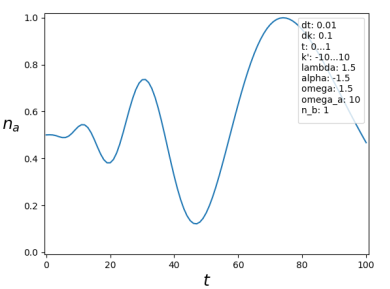
\includegraphics[width=0.65\linewidth]{pictures/result_first_1.png}
    \caption{Осциллирующее поведение}
    \label{fig:fr_oscillation}
\end{figure}

Такой результат сложно~объяснить с точки~зрения когнитивной психологии, поскольку экспериментов с таким
эффектом найти не удалось.
Результат моделирования приведенный на рисунке~\ref{fig:fr_oscillation} можно описать как "метание"
агента из одного выбора к другому, когда человеку через некоторое время кажется, что он сделал фатальную
ошибку в выборе, но такое объяснение, к сожалению, не удалось привести из-за отсутствия реальных
экспериментов.
Помимо необъяснимости полученного результата, приведенного на рисунке~\ref{fig:fr_oscillation}, стоит
отметить отсутствие комплексной плоскости на графике, поскольку присутствие комплексной составляющей
в результате моделирования дает предпосылки к ошибке вычисления, а это необходимо учитывать при моделировании.
Такой же результат без комплексной плоскости необходимо отметить на следующем графике (рисунок~\ref{fig:fr_next}).
\begin{figure}[h!]
    \centering
    \captionsetup{justification=centering}
    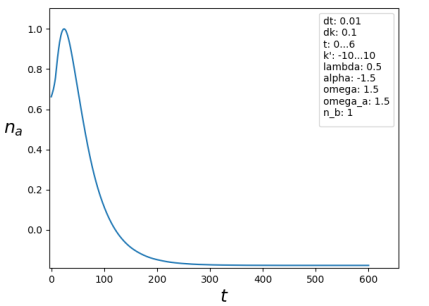
\includegraphics[width=0.7\linewidth]{pictures/result_first_2.png}
    \caption{Экспоненциальное затухание когнитивного возбуждения с пичком}
    \label{fig:fr_next}
\end{figure}

На~рисунке~\ref{fig:fr_next}~происходит~некоторое~временное возбуждение с последующим затуханием,~поведение
которого~также объясняется комплексным или отрицательным параметром плотности $g$.
В когнитивистике это поведение можно объяснить как ситуацию с отрицанием противоположной точки зрения.
Когда среда начинает воздействовать на сознание противоречивой информацией, вызывая у человека когнитивный
диссонанс, проявляющаяся ответной реакцией в виде пичка на графике, но через некоторое время ответная
реакция сознания индивида постепенно затухает, иначе говоря индивид переходит к состноянию среды.

Более правильным поведением является случай с параметром плотности $g = 1$, по причине отсутствия
комплексной составляющей в результатах модели, иначе говоря $n_{a} \in \mathbb{R}$.
Конечно, данное действие не является правильным с точки зрения вычислений, поскольку в таком случае
коммутатор в уравнении~\eqref{dynamic_comm} не равняется нулю, а это значит что оператор рождения и
уничтожения агента не коммутируют, чего не должно происходить.
Поведение при $g = 1$ показано на рисунке~\ref{fig:fr_real_g_15}.
\begin{figure}[h!]
    \centering
    \captionsetup{justification=centering}
    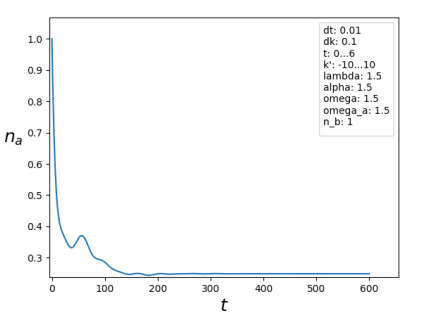
\includegraphics[width=0.7\linewidth]{pictures/result_first_4.png}
    \caption{Экспоненциальное затухание при вещественном значении параметра $g$}
    \label{fig:fr_real_g_15}
\end{figure}
Как видно из рисунка~\ref{fig:fr_real_g_15} его поведение схоже с марковской квантово-подобной моделью,
про которую было сказано ранее, приведенной в уравнении~\eqref{na_bagarello} и на рисунке~\ref{fig:at_baga}.
С точки зрения квантовой когнитивистики это поведение было описано ранее в других
работах~\citep{bagarello2015quantum,bagarello2018quantum}.

В залючении этой части необходимо уточнить причины проблемы присутствия комплексной составляющей в модели.
Проблема заключается не только в том, что параметр плотности $g$ вносит комплексную составляющую в оператор
принятия решения $n_{a} \in \mathbb{C}$, но и в том, что поскольку даже отнормировав основные уравнения
по $g$, из-за чего в коммутаторе~\eqref{dynamic_comm} он исчезает, отрицаельными или комплексными окажутся
другие параметры, так как необходимо соблюдать коммутационные соотношения.
Решением этой проблемы может быть поиск аналитического способа, но в данной работе этого сделать не удалось.
В таком случае необходимо найти приближенный вид аналитического решения, что может быть осуществимо.

%%%%%%%%%%%%%%%%%%%%%%%%%%%%%%%%%%%%%%%%%%%%%%%%%%%%%%%%%%%%%%%%%%%%%%%%%%%%%%%%%%%%%%%%%%%%%%%%%%%%
%%%%%%%%%%%%%%%%%%%%%%%%%%%%%%%%%%%%%%%%%%%%%%%%%%%%%%%%%%%%%%%%%%%%%%%%%%%%%%%%%%%%%%%%%%%%%%%%%%%%
\section{Второй способ моделирования}

Для приближенного аналитического решения необходимо найти численное решение уравнения для оператора
агента $a(t), a^{\dagger}(t)$.
В основу численного решения было взято нормированное по $g$ уравнение~\eqref{dotat_norm}, вывод которого
подробно приведен в приложении.
\begin{equation}\label{dotat_norm}
    \dot{a}(t) =
    -i \omega^{'}_{a} a(t)
    -i \lambda \int \frac{b(k)e^{-i \omega k t}}{\sqrt{k^{2} + \alpha^2}} dk
    -\frac{\lambda^{2} \pi}{\alpha} \int_{0}^{t} a(\tau) e^{- \alpha \omega (t - \tau)} d\tau
\end{equation}
Как видно из уравнения~\eqref{dotat_norm} в нем отсутствует параметр плотности, а это значит его
задавать не нужно.
Применяем итерационный метод решения для уравнения~\eqref{dotat_norm}, который имеет вид:
\begin{multline}
    a(t + \Delta t) =
    -i \omega^{'}_{a} a(t) \Delta t
    -i \lambda \int \frac{b(k)e^{-i \omega k t}}{\sqrt{k^{2} + \alpha^2}} dk \Delta t \\
    -\frac{\lambda^{2} \pi}{\alpha} \int_{0}^{t} a(\tau) e^{- \alpha \omega (t - \tau)} d\tau \Delta t
    - a(t)
\end{multline}
Все параметры в этом уравнении задаются случайным способом в диапазоне вещественных чисел кроме одного.
Этим параметром является оператор резервуара $b(k), b^{\dagger}(k)$, который задается в области
комплексных значений.
В ходе расчетов было выяснено, что большую зависимость оператор агента $a(t), a^{\dagger}(t)$ проявляет
в зависимости от оператора резервуара $b(k), b^{\dagger}(k)$, а это зачит необходимо продумать
приближенные значения этого параметра в итерационном методе решения.
Поскольку известно, что операторы рождения и уничтожения комплексно-сопряженные между собой, то значит
можно предположить отличия между оператором рождения и уничтожения только знаком комплексной составляющей.
Помимо этого, параметр $b(k), b^{\dagger}(k)$ не просто число, а некоторая зависимость от параметра $k$.
Такая зависимость может иметь большое количество вариантов, из которых выявить основные не получится.
Моделирование оператора рождения и уничтожения резервуара $b(k), b^{\dagger}(k)$ нетривиальная задача,
которая требует отдельного рассмотрения, но без него невозможны дальнейшие действия.
В таком случае оператор рождения и уничтожения для резервуара были приняты равными константе
$b(k) = b, b^{\dagger}(k) = b^{\dagger}$, при этом они должны быть комплексно-сопряженными.

После численного решения оператора рождения и уничтожения агента $a(t), a^{\dagger}(t)$ остается
вопрос о проверке результатов.
Проверка результатов может быть проведена с помощью коммутационных соотношений $[a(t), a^{\dagger}(t)] = 1$,
которые уже были показаны в данной работе.
Эти коммутационные соотношения работают только для $a(t), a^{\dagger}(t)$, но не для
$\dot{a}(t), \dot{a}^{\dagger}(t)$, поэтому нужно найти хотя бы приближенное аналитическое решение.
Хорошим показателем правильного моделирования является отсутствие комплексного составляющего в результате
получения оператора принятия решения $n_{a}$, но для данного метода решения этого можно не делать,
поскольку параметры задаются вещественными в начале моделирования.
Получив итерационным методом оператор рождения и уничтожения агента $a(t), a^{\dagger}(t)$, можно
перейти к численному результату оператора принятия решения $n_{a}$.
Результаты численного решения оператора принятия решения преведны в следующей части главы.

%%%%%%%%%%%%%%%%%%%%%%%%%%%%%%%%%%%%%%%%%%%%%%%%%%%%%%%%%%%%%%%%%%%%%%%%%%%%%%%%%%%%%%%%%%%%%%%%%%%%
%%%%%%%%%%%%%%%%%%%%%%%%%%%%%%%%%%%%%%%%%%%%%%%%%%%%%%%%%%%%%%%%%%%%%%%%%%%%%%%%%%%%%%%%%%%%%%%%%%%%
\section{Результаты вычисления вторым способом}

Для данного способа решения полученные данные оказались более правильными, поскольку комплексная составляющая
отсутствовала для всех результатов моделирования.
Результаты моделирования хорошо показывают проявление немарковского процесса, эффекта влияния "памяти"
на принятие решения, постепенный переход к равновесию в информационном резервуаре.
Разработанная модель очень просто сводится к результатам марковской квантово-подобной модели~\citep{bagarello2018quantum},
если задать степень влияния осцилляций на модель достаточно слабыми, а параметр $\alpha$ задать гораздо
больше чем в два раза частотной характеристики $\omega_{a}$, что как раз приведено на рисунке~\ref{fig:sr_mark}.
\begin{figure}[h!]
    \centering
    \captionsetup{justification=centering}
    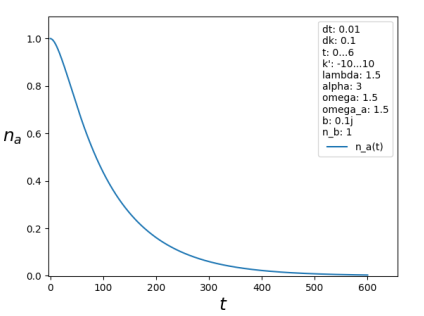
\includegraphics[width=0.7\linewidth]{pictures/result_second_1.png}
    \caption{Марковское приближение при малых осцилляциях резервуара и $\alpha = 3$}
    \label{fig:sr_mark}
\end{figure}

Для сравнения приведенного результата на рисунке~\ref{fig:sr_mark} с марковской квантово-подобной
моделью принятия решения можно обратиться к рисунку~\ref{fig:at_baga}.
Этот результат не представляет интереса в даннной работе, поскольку такие результаты обсуждались в других работах.
Другой случай показывает влияние немарковского процесса на поведение агента при воздействии резервуара,
который приведен на рисунке~\ref{fig:sr_nomark}.
\begin{figure}[h!]
    \centering
    \captionsetup{justification=centering}
    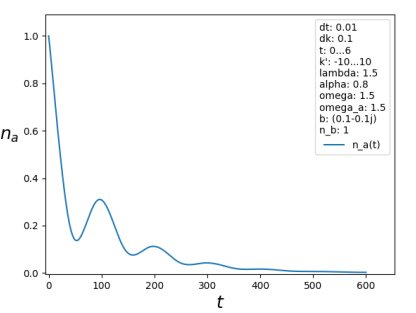
\includegraphics[width=0.7\linewidth]{pictures/result_second_2.png}
    \caption{Немарковское поведение при малых осцилляциях резервуара и $\alpha = 0.8$}
    \label{fig:sr_nomark}
\end{figure}

Как видно из рисунка~\ref{fig:sr_nomark} агент стремится к начальному решению через некоторое время
равному $t = 100, 200, 300$, происходят осциляции с затуханием.
Такое поведение, с точки зрения конитивистики, объясняется как "когнитивный шум" и наблюдается в
социальных сетях при воздействии информационной среды сообщества на участника этого сообщества.
Как видно из рисунка~\ref{fig:sr_mark} и рисунка~\ref{fig:sr_nomark} немарковский процесс может
переходить в марковский, в случае малых величин оператора рождения(уничтожения) резервуара $b, b^{\dagger}$
и параметра $\alpha$ больше частотной характеристики агента $\omega_{a}$.
Было обнаружено, что при уменьшении параметра $\alpha$ относительно частотной характеристики $\omega_{a}$,
увеличивается частота осциляций модели, что в данном случае наблюдается на рисунке~\ref{fig:sr_more_oscillation}.
\newpage
\begin{figure}[h!]
    \centering
    \captionsetup{justification=centering}
    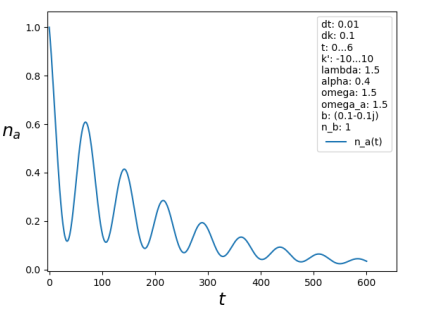
\includegraphics[width=0.7\linewidth]{pictures/result_second_3.png}
    \caption{Немарковское поведение при малых осцилляциях резервуара и $\alpha = 0.4$}
    \label{fig:sr_more_oscillation}
\end{figure}
Необходимо отметить зависимость диапазона моделирования от величины модуля оператора рождения(уничтожения)
резевуара $\arrowvert b \arrowvert, \arrowvert b^{\dagger} \arrowvert$.
Поскольку диапазон принятия решения находится в пределах от 0 до 1, то и параметры модели должны быть
подобраны таким образом, чтобы в результате соответсвовать этим ограничениям.
Поэтому сумма модулей оператора рождения и уничтожения резервуара не должны превышать 1, иначе говоря
сумма радиусов их векторов на комплексной плоскости не должны первышать 1.
На рисунке~\ref{fig:sr_more_oscillation} можно заметить, что нижние полупериоды осцилляций модели достигают
минимума постепенно, по закону гауссовой функции.
Это поведение можно наблюдать в физике при изучении степени пространственной когерентности реальных
лазерных источников в интерверометре Юнга, когда темные полосы интерференционной картины "засвечены"
нескоррелированными фотонами.
Такое поведение моделируется если сумма действительной части оператора рождения и уничтожения резервуара
близка по сумме к 1.
Более наглядное представление этого поведения представлено на рисунке~\ref{fig:sr_gauss}.
\begin{figure}[h!]
    \centering
    \captionsetup{justification=centering}
    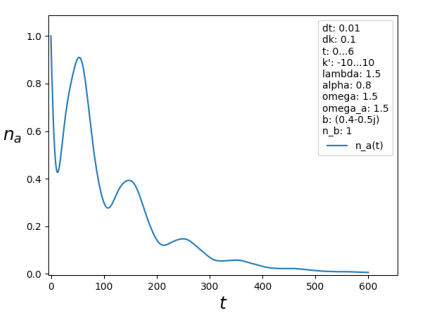
\includegraphics[width=0.7\linewidth]{pictures/result_second_4.png}
    \caption{Немарковское поведение с возвышенными нижними полупериодами осцилляций}
    \label{fig:sr_gauss}
\end{figure}
Песледний вопрос в этой части касается приближенного аналитического вида модели принятия решения.
Для решения вопроса необходимо описать основные уравнения, которые будут составлять характер модели.
Первое что необходимо отметить, это присутствие осцилляций, характер которых может описать уравнение
косинуса.
Поскольку косинус находится в пределе от -1 до 1, то его значения нужно увеличить на единицу.
Осцилляции в модели со временем затухают и их характер затухания необходимо подбирать.
Для уравнения затухания было выбрано уравнение экспоненты в отрицательной степени, которая составляет
проезведение с уравнением косинуса.
В вышеприведенных результатах поведение агента стремится к покою(к 0) и это значит присутствие экспоненты
в знаменателе для всего полученного аналитического решения.
Окончательный результат этой приближенной модели представлен следующим образом:
\begin{equation}
    f(t) = \frac{cos(tx - y)*e^{-tz} + 1}{e^{t}},
\end{equation}
где $x$ - параметр частоты, $y$ - параметр сдвига, $z$ - параметр затухания осцилляций, $t$ - время.
Для демонстрации результатов поиска приближенного решения оператора принятия решения следует привести
уравнения с подобраными параметрами.
Первое уравнение имеет следующий вид:
\begin{equation}
    f(t) = \frac{cos(10*t/1.645 - 10)*e^{-t*0.3} + 1}{e^{t}},
\end{equation}
и его результат с приведенным немарковским поведением модели при сильных осциллциях и их "сильных" минимумов~\ref{fig:sr_proba_1}.
\begin{figure}[h!]
    \centering
    \captionsetup{justification=centering}
    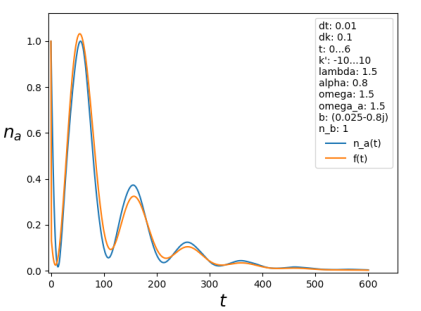
\includegraphics[width=0.7\linewidth]{pictures/result_second_5.png}
    \caption{Поведение модели и приблеженного аналитического решения}
    \label{fig:sr_proba_1}
\end{figure}
Второе уравнение имеет следующий вид:
\begin{equation}
    f(t) = \frac{cos(10*t/1.645 - 9.5)*e^{-t*0.8} + 1}{e^{t}},
\end{equation}
где его результат с вышеприведенным поведением приведен на следующем рисунке~\ref{fig:sr_proba_2}.
\newpage
\begin{figure}[h!]
    \centering
    \captionsetup{justification=centering}
    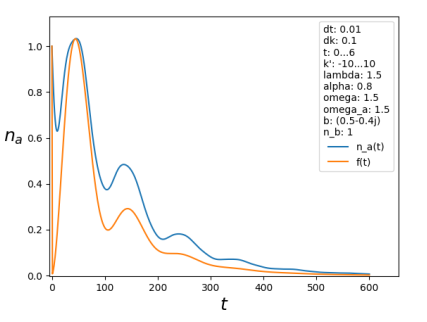
\includegraphics[width=0.7\linewidth]{pictures/result_second_6.png}
    \caption{Поведение модели и приблеженного аналитического решения с другими параметрами}
    \label{fig:sr_proba_2}
\end{figure}

Коммутационное соотношение из приближенного уравнения взять не получится, поскольку отсутствует
оператор рождения(уничтожения) в слагаемых.
Но основная задача данной работы решена, поскольку была получена модель, описывающая эмпирические
данные в социальных сетях.

    % Заключение
    %! Author = jaroslav
%! Date = 22.04.20
\conclusion

В ходе проведенной работы было изучено большинство когнитивных эффектов возникающие в условиях неопределенности.
На основании изученных работ, была разработана модель принятия решения агентом с учетом его взаимодействия
(обмена информацией) с внешним окружением, описываемым резервуаром.
Когнитивное состояние агента в рассматриваемой модели описывается вектором в Гильбертовом пространстве,
а процесс ПР в представлении вторичного квантования характеризуется операторами рождения $a^{\dagger}$
и уничтожение $a$, которые определяют динамику ПР.
Наблюдаемой величиной в рассматриваемой задаче является оператор принятия решения $n_{a} = a^{\dagger} a$,
который усреднялся по когнитивным состояниям ПР и определяет основную динамику данного процесса.
В зависимости от типа внешнего информационного резервуара процесс принятия решения агентом имел марковский
и немарковский характер.
Проведен аналитический и численный анализ модели динамического принятия решения агентом с учетом как
марковости, так и не марковости резервуара, имеющего бесконечное число степеней свободы.
Было показано, что влияние резервуара на агента ПР приводит к различным режимам затухания вероятности
принятия решения, имеющим экспоненциальный~характер в случае марковости процесса и осциллирующий
характер~в~случае немарковости процесса.
Переход от марковского к немарковскому~процессу осуществляется через изменение параметров ядра
взаимодействия $g(k)$ агента ПР и внешнего информационного окружения.
Был проведен анализ зависимости динамики принятия решения агентом от вводимых параметров процесса,
который позволил выявить, что является режимом существенно~осциллирующего немарковоского взаимодействия
агента ПР с резервуаром.
Так как немарсковский процесс имеет сложную по своей структуре динамику, в работе был проведен аналитический
анализ полученных результатов, который позволил получить аналитическое решение рассматриваемой модели.
Данное аналитическое решение хорошо согласуется с полученным численный моделированием модели.

    % Список сокращений и условных обозначений
%    \printnomenclature

    % Не добавлять длинное тире в качестве разделителя
%    \newcommand\BibDash{}
    % Выделять курсивом
%    \let\BibEmph=\emph
%    \bibliographystyle{unsrt}
%    \bibliographystyle{ugost2008n}
    \bibliographystyle{ugost2003}

    % Список литературы
    \bibliography{sources}

    % Приложения
    \appendix
    %! Author = jaroslav
%! Date = 03.03.20
\chapter{Основные аналитические методы построения модели}

Рассмотрим резервуар~с бесконечным числом степеней свободы $k$ частицы которого описываются~бесконечным~числом
оператора рождения(уничтожения) $b^\dagger(b)$.
Данный резервуар определяет информационную среду,~с~которой~взаимодействует агент ПР.
ПР агента в представлении вторичного~квантования характеризуется операторами рождения (уничтожения)
$a^\dagger(a)$ в Гильбертовом пространстве.
Эти операторы должны подчиняться следующим коммутационным соотношениям:
$
[\hat{a}, \hat{a}^{\dagger}] = 1,
[\hat{b}(k), \hat{b}^{\dagger}(k)] = \delta (k-k')
$
в то время как все остальные коммутаторы предполагаются равными нулю.
Полный Гамильтониан расматриваемой системы взаимодействия внешнего информационного поля (резервуара) и агента ПР имеет вид:

\begin{multline}\label{H}
H_f = \hbar \omega_a a^{\dagger} a + \hbar \lambda \int g(k) (b^{\dagger}(k) a + a^{\dagger} b(k)) d^{D}(k) \\
+ \hbar \lambda \int g(k) (b^{\dagger}(k) a + a^{\dagger} b(k)) d^{D}(k),
\end{multline}

где ${\omega_a}$($\omega_b$) - частотная характеристика~агента(резервуара) соотвественно; $\lambda$
- коэффициент взаимодействия агента и резервуара; $g(k)$ - ядро, определеяющее сруктуру резервуара;
$D$ - размерность пространства резервуара.
В данной работе мы ограничеваемся одномерным резервуаром $D=1$.
Ядро резервуара $g(k)$ определяющее взаимодействие информационной среды и агента ПР в данной работе имеет вид:

\begin{equation}
    g^{2}(k) = \frac{g}{k^{2} + \alpha^{2}},
\end{equation}

Таким~образом, отнормировав~уравнение \eqref{H} на константу $g$, определяющая ширину распределения
ядра мы получим:

\begin{equation}\label{H'}
H' =  \omega^{'}_a a^{\dagger} a +  \int \omega^{'}_{R}(k) b^{\dagger}(k) b(k) dk+ \lambda \int \frac{(b^{\dagger}(k) a + a^{\dagger} b(k))}{\sqrt{k^{2} + \alpha^{2}}} dk,
\end{equation}
где $\omega^{'}_a = \omega_a/g$, $\omega^{'}_{R}(k) = \omega_{R}(k)/g$.

Решая уравнение Гейзенберга  $i\frac{\partial f}{\partial t}=[f,H]$, $ f \in a(a^{\dagger})$ и
$b(b^{\dagger})$ можно получить операторные уравнения для операторов уничтожения $a$ и $b$.
Принимая во внимание коммутационные соотношение для операторов $a$ и $b$, решение уравнение
Гейзенберга для оператора $b$ имеет вид:

\begin{equation}\notag
\begin{split}
    i \hbar \frac{\partial b(k,t)}{\partial t} & = [b(k,t), H] = \\
    & = \hbar \omega^{'}_a b(k,t) a^{\dagger}(t) a(t) + \hbar \int \omega^{'}_{R}(k) b(k,t) b^{\dagger}(k,t) b(k,t) d^{D}(k) + \\
    & + \hbar \lambda \int \frac{(b(k,t) b^{\dagger}(k,t) a(t) + b(k,t) a^{\dagger}(t) b(k,t))}{\sqrt{k^{2} + \alpha^{2}}} d^{D}(k) - \\
    & - \hbar \omega^{'}_a a^{\dagger}(t) a(t) b(k,t) - \hbar \int \omega^{'}_{R}(k) b^{\dagger}(k,t) b(k,t) b(k,t) d^{D}(k) - \\
    & - \hbar \lambda \int \frac{(b^{\dagger}(k,t) a(t) b(k,t) + a^{\dagger}(t) b(k,t) b(k,t))}{\sqrt{k^{2} + \alpha^{2}}} d^{D}(k) = \\
    & = xx' + yy' + zz' = \hbar \omega^{'}_{R}(k) b(k,t) + \hbar \lambda \frac{a(t)}{\sqrt{k^{2} + \alpha^{2}}}
\end{split}
\end{equation}
где
\begin{equation}\notag
\begin{split}
    xx' & = \hbar \omega^{'}_a b(k,t) a^{\dagger}(t) a(t) - \hbar \omega^{'}_a a^{\dagger}(t) a(t) b(k,t) = \\
    & = \cancel{\hbar \omega^{'}_a a^{\dagger}(t) b(k,t) a(t)} - \hbar \omega^{'}_a \underbrace{[a^{\dagger}(t), b(k,t)]}_{0} a(t) - \\
    & - \hbar \omega^{'}_a a^{\dagger}(t) \underbrace{[a(t), b(k,t)]}_{0} - \cancel{\hbar \omega^{'}_a a^{\dagger}(t) b(k,t) a(t)} = \\
    & = 0
\end{split}
\end{equation}
\begin{equation}\notag
\begin{split}
    yy' & = \hbar \int \omega^{'}_{R}(k) b(k,t) b^{\dagger}(k,t) b(k,t) d^{D}(k) - \\
    & - \hbar \int \omega^{'}_{R}(k) b^{\dagger}(k,t) b(k,t) b(k,t) d^{D}(k) = \\
    & = \hbar \int \omega^{'}_{R}(k) \Bigl([b(k,t), b^{\dagger}(k,t)] b(k,t) + \\
    & + \cancel{b^{\dagger}(k,t) b(k,t) b(k,t)} - \cancel{b^{\dagger}(k,t) b(k,t) b(k,t)} \Bigr) d^{D}(k) = \\
    & = \hbar \int \omega^{'}_{R}(k) \delta (k-k') b(k,t) d^{D}(k) = \hbar \omega^{'}_{R}(k') b(k',t)
\end{split}
\end{equation}
\begin{equation}\notag
\begin{split}
    zz' & = \hbar \lambda \int \frac{(b(k,t) b^{\dagger}(k,t) a(t) + b(k,t) a^{\dagger}(t) b(k,t))}{\sqrt{k^{2} + \alpha^{2}}} d^{D}(k) - \\
    & - \hbar \lambda \int \frac{(b^{\dagger}(k,t) a(t) b(k,t) + a^{\dagger}(t) b(k,t) b(k,t))}{\sqrt{k^{2} + \alpha^{2}}} d^{D}(k) = \\
    & = \hbar \lambda \int \frac{[b(k,t), b^{\dagger}(k,t)] a(t) + \cancel{b^{\dagger}(k,t) b(k,t) a(t)}}{\sqrt{k^{2} + \alpha^{2}}} d^{D}(k) - \\
    & - \hbar \lambda \int \frac{\overbrace{[a^{\dagger}(t), b(k,t)]}^{0} b(k,t) + \cancel{a^{\dagger}(t) b(k,t) b(k,t)}}{\sqrt{k^{2} + \alpha^{2}}} d^{D}(k) - \\
    & - \hbar \lambda \int \frac{b^{\dagger}(k,t) \overbrace{[a(t), b(k,t)]}^{0} + \cancel{b^{\dagger}(k,t) b(k,t) a(t)} + }{\sqrt{k^{2} + \alpha^{2}}} d^{D}(k) = \\
    & + \hbar \lambda \int \frac{\cancel{a^{\dagger}(t) b(k,t) b(k,t)}}{\sqrt{k^{2} + \alpha^{2}}} d^{D}(k) = \\
    & = \hbar \lambda \int \frac{[b(k,t), b^{\dagger}(k,t)] a(t)}{\sqrt{k^{2} + \alpha^{2}}} d^{D}(k) = \hbar \lambda \int \frac{\delta (k-k') a(t)}{\sqrt{k^{2} + \alpha^{2}}} d^{D}(k) = \\
    & = \hbar \lambda \frac{a(t)}{\sqrt{k^{2} + \alpha^{2}}}
\end{split}
\end{equation}

Решение уравнение Гейзенберга для оператора $a$:
\begin{equation}\notag
\begin{split}
    i \hbar \frac{\partial a(t)}{\partial t} & = [a(t), H] = \\
    & = \hbar \omega^{'}_a a(t) a^{\dagger}(t) a(t) + \hbar \int \omega^{'}_{R}(k) a(t) b^{\dagger}(k,t) b(k,t) d^{D}(k) + \\
    & + \hbar \lambda \int \frac{(a(t) b^{\dagger}(k,t) a(t) + a(t) a^{\dagger}(t) b(k,t))}{\sqrt{k^{2} + \alpha^{2}}} d^{D}(k) - \\
    & - \hbar \omega^{'}_a a^{\dagger}(t) a(t) a(t) - \hbar \int \omega^{'}_{R}(k) b^{\dagger}(k,t) b(k,t) a(t) d^{D}(k) - \\
    & - \hbar \lambda \int \frac{(b^{\dagger}(k,t) a(t) a(t) + a^{\dagger}(t) b(k,t) a(t))}{\sqrt{k^{2} + \alpha^{2}}} d^{D}(k) = \\
    & = xx' + yy' + zz' = \hbar \omega^{'}_a a(t) + \hbar \lambda \int \frac{b(k,t)}{\sqrt{k^{2} + \alpha^{2}}} d^{D}(k)
\end{split}
\end{equation}

где
\begin{equation}\notag
\begin{split}
    xx' & = \hbar \omega^{'}_a a(t) a^{\dagger}(t) a(t) - \hbar \omega^{'}_a a^{\dagger}(t) a(t) a(t) = \\
    & = \hbar \omega^{'}_a \underbrace{[a(t), a^{\dagger}(t)]}_{1} a(t)
    + \cancel{\hbar \omega^{'}_a a^{\dagger}(t) a(t) a(t)}
    - \cancel{\hbar \omega^{'}_a a^{\dagger}(t) a(t) a(t)} = \\
    & = \hbar \omega^{'}_a a(t) \\
    yy' & = \hbar \int \omega^{'}_{R}(k) \overbrace{a(t) b^{\dagger}(k,t) b(k,t)}^{= b^{\dagger}(k,t) a(t) b(k,t)} d^{D}(k) \\
    & - \hbar \int \omega^{'}_{R}(k) \overbrace{b^{\dagger}(k,t) b(k,t) a(t)}^{= b^{\dagger}(k,t) a(t) b(k,t)} d^{D}(k) = 0 \\
    zz' & = \hbar \lambda \int \frac{(a(t) b^{\dagger}(k,t) a(t)
    + a(t) a^{\dagger}(t) b(k,t))}{\sqrt{k^{2} + \alpha^{2}}} d^{D}(k) - \\
    & - \hbar \lambda \int \frac{(b^{\dagger}(k,t) a(t) a(t)
    + a^{\dagger}(t) b(k,t) a(t))}{\sqrt{k^{2} + \alpha^{2}}} d^{D}(k) = \\
\end{split}
\end{equation}
\begin{equation}\notag
\begin{split}
    zz' & = \hbar \lambda \int \frac{\overbrace{[a(t), b^{\dagger}(k,t)]}^{0} a(t) + \cancel{b^{\dagger}(k,t) a(t) a(t)}}{\sqrt{k^{2} + \alpha^{2}}} d^{D}(k) + \\
    & + \hbar \lambda \int \frac{[a(t), a^{\dagger}(t)] b(k,t) + \cancel{a^{\dagger}(t) a(t) b(k,t)}}{\sqrt{k^{2} + \alpha^{2}}} d^{D}(k) - \\
    & - \hbar \lambda \int \frac{\cancel{b^{\dagger}(k,t) a(t) a(t)} - a^{\dagger}(t) \overbrace{[a(t), b(k,t)]}^{0} +
    \cancel{a^{\dagger}(t) a(t) b(k,t)} }{\sqrt{k^{2} + \alpha^{2}}} d^{D}(k) = \\
    & = \hbar \lambda \int \frac{[a(t), a^{\dagger}(t)] b(k,t)}{\sqrt{k^{2} + \alpha^{2}}} d^{D}(k) =
    \hbar \lambda \int \frac{b(k,t)}{\sqrt{k^{2} + \alpha^{2}}} d^{D}(k)
\end{split}
\end{equation}


В результате, мы имеем следующий вид операторных уравнений для операторов уничтожения $a$ и $b$

{\large
\begin{equation}\label{syst}
\begin{cases}
    & \dot{a}(t) = -i \omega^{'}_a a(t) - i \lambda \int \frac{b(k,t)}{\sqrt{k^{2} + \alpha^{2}}} d^{D}(k) \\
    & \dot{b}(k,t) = -i \omega^{'}_{R}(k) b(k,t) -i \lambda \frac{a(t)}{\sqrt{k^{2} + \alpha^{2}}}
\end{cases}
\end{equation}}


Решение системы ищется адиабатически исключая резервуар.
То есть, в начале решается второе уравнение системы \eqref{syst} на ${b}(k,t) $, а затем его решение
подставляется в первое уравнение на $\dot{a}(t)$.
Физически это означает, что сперва формируется резервуар, а лишь затем он формирует свойства агента.
Уравнение на ${b}(k,t)$ является неоднородным дифференциальным уравнением, решение которого имеет
вид суммы соотвествующего линейного однородного дифференциального уравнения (ЛОДУ) и частоного решения
неоднородного дифференциального уравнения (ЛНДУ).
Решение ЛОДУ имеет вид:
\begin{equation}\label{LODY}
\begin{split}
    & \frac{\partial b(k,t)}{\partial t} = -i \omega^{'}_{R}(k) b(k,t); \\
    & b(k,t) = Ce^{-i \omega^{'}_{R}(k) t} \\
\end{split}
\end{equation}

В общем случае $C = C(t)$ и для определения данной функции необходимо подставить \eqref{LODY} в
соотвествующее ЛНДУ, таким образом:

\begin{equation}\notag
    (C(t)e^{-i \omega^{'}_{R}(k) t})^{'}_{t} = -i \omega^{'}_{R}(k) C(t)e^{-i \omega^{'}_{R}(k) t} -i \lambda \frac{a(t)}{\sqrt{k^{2} + \alpha^{2}}}
\end{equation}
\begin{equation}\label{LNDY}
    C(t) = -i \lambda \int \frac{a(t)e^{i \omega^{'}_{R}(k) t}}{\sqrt{k^{2} + \alpha^{2}}} dt + C_{1}
\end{equation}

Объединяя \eqref{LODY} и \eqref{LNDY} получим решение оператора ${b}(k,t)$ в следующем виде:

\begin{equation}\notag
b(k,t) = b(k)e^{-i \omega^{'}_{R}(k) t} -i \lambda \int_{0}^{t} \frac{a(\tau)e^{-i \omega^{'}_{R}(k) (t-\tau)}}{\sqrt{k^{2} + \alpha^{2}}} d\tau \\
\end{equation}
Данное решение легко проверить, подвставив его в \eqref{syst}.
\begin{multline}\notag
\Biggl( b(k)e^{-i \omega^{'}_{R}(k) t} -i \lambda \int_{0}^{t} \frac{a(\tau)e^{-i \omega^{'}_{R}(k) (t-\tau)}}{\sqrt{k^{2} + \alpha^{2}}} d\tau \Biggr)^{'}_{t} =  \\
= b(k) \Bigl( e^{-i \omega^{'}_{R}(k) t} \Bigr)^{'}_{t} - i \lambda \Biggl( \int_{0}^{t} \frac{a(\tau)e^{-i \omega^{'}_{R}(k) (t-\tau)}}{\sqrt{k^{2} + \alpha^{2}}} d\tau \Biggr)^{'}_{t} = \\
= -i \omega^{'}_{R}(k) \underbrace{b(k)e^{-i \omega^{'}_{R}(k) t}}_{b(k,0) = b(k,t)} -i \lambda \frac{a(t) \cancel{e^{-i \omega^{'}_{R}(k) (t-t)}}}{\sqrt{k^{2} + \alpha^{2}}} = \\
= -i \omega^{'}_{R}(k) b(k,t) -i \lambda \frac{a(t)}{\sqrt{k^{2} + \alpha^{2}}}
\end{multline}


Мы принимаем $\omega^{'}_{R}(k) = \omega k$ опираясь на известное волновое соотношение в оптике.
С учетом того, что аналитически решение интеграла имеет вид:
\begin{equation}\notag
    \int \frac{e^{-i \omega k (t - \tau)}}{k^{2} + \alpha^{2}} dk = \frac{\pi}{\alpha} e^{-\alpha \omega (t - \tau)},
\end{equation}
то в адиабатическом приближении решение системы \eqref{syst} имеет вид:
\begin{equation}\label{a}
    \dot{a}(t) =
    -i \omega^{'}_{a} a(t)
    -i \lambda \int \frac{b(k)e^{-i \omega k t}}{\sqrt{k^{2} + \alpha^2}} dk
    -\frac{\lambda^{2} \pi}{\alpha} \int_{0}^{t} a(\tau) e^{- \alpha \omega (t - \tau)} d\tau
\end{equation}

Решить данное интегрально-операторное уравнение явно не получится из-за специфики данного уравнения,
поэтому дальнейший анализ модели осуществлялся численно.
В работе использовался итерационный метод для решения данного уравнения и поиска наблюдаемой
величина $n_a=\langle{a^{\dagger}(t)a(t)\rangle}$, где усреденение проводится по когнитивным состониям ПР.
Для численного решения переведем интегральное уравнение в дифференциальное, таким образом:
\begin{equation}\label{dot_na}
\frac{\partial n_{a}(t)}{\partial t}
= \frac{\partial (a^{\dagger}(t) a(t))}{\partial t}
= \frac{\partial a^{\dagger}(t)}{\partial t}a(t) + a^{\dagger}(t)\frac{\partial a(t)}{\partial t}
= \dot{a}^{\dagger}(t) a(t) + a^{\dagger}(t) \dot{a}(t).
\end{equation}
Используя уравнение \eqref{a} мы можем получить следующие соотношения:
\begin{multline}\notag
    \dot{a}^{\dagger}(t) a(t)=
    i \omega^{'}_{a} a^{\dagger}(t) a(t)
    + i \lambda \int \frac{b^{\dagger}(k) a(t) e^{i \omega k t}}{\sqrt{k^{2} + \alpha^2}} dk \\
    -\frac{\lambda^{2} \pi}{\alpha} \int_{0}^{t} a^{\dagger}(\tau) a(t) e^{- \alpha \omega (t - \tau)} d\tau
\end{multline}
\begin{multline}\notag
    a^{\dagger}(t) \dot{a}(t) =
    -i \omega^{'}_{a} a^{\dagger}(t) a(t)
    -i \lambda \int \frac{a^{\dagger}(t) b(k)e^{-i \omega k t}}{\sqrt{k^{2} + \alpha^2}} dk \\
    - \frac{\lambda^{2} \pi}{\alpha} \int_{0}^{t} a^{\dagger}(t) a(\tau) e^{- \alpha \omega (t - \tau)} d\tau
\end{multline}
Подстовляя данные выражения в исходное соотношение \eqref{dot_na} можем получить дифференциальное уравнение наблюдаемой величины $n_a(t)$ в следующем виде:
\begin{multline}
    \frac{\partial n_{a}(t)}{\partial t} =
    i \lambda \int \frac{(b^{\dagger}(k) a(t) e^{i \omega k t} - a^{\dagger}(t) b(k)e^{-i \omega k t})}{\sqrt{k^{2} + \alpha^2}} dk - \\
    - \frac{\lambda^{2} \pi}{\alpha} \int_{0}^{t} e^{- \alpha \omega (t - \tau)} \overbrace{(a^{\dagger}(\tau) a(t) + a^{\dagger}(t) a(\tau))}^{n_{a}(t) \delta(t-\tau) + n_{a}(t) \delta(t-\tau)} d\tau
\end{multline}
в простом виде выражение \eqref{dot_na} можно переписать следующим образом:
\begin{equation}\label{na}
    \frac{\partial n_{a}(t)}{\partial t} =
    i \lambda \int \frac{(b^{\dagger}(k) a(t) e^{i \omega k t} - a^{\dagger}(t) b(k) e^{-i \omega k t})}{\sqrt{k^{2} + \alpha^2}} dk
    - 2 \frac{\lambda^{2} \pi}{\alpha} n_{a}(t)
\end{equation}

Данное выражение позволяет отследить как динамику процесса принятие решение у агента.
Третье слогаемое данного выражение имеет смысл ассимтотической стабилизации, при которой $n_a(t)$ уменьшается со временем.
В этом случае исключая второе слогаемое мы получим результат описанный в работе
$n_a(t)=n_{a}e^{-\frac{-2\lambda^2\pi}{\alpha}t}$ описывающий изночально пустой резервуар.
Второе слагаеме в выражении \eqref{na} описывает немарковское воздействие резервуара на агента ПР.
Для численного анализа данного слогаемого необходимо определить $(b^{\dagger}(k) a(t)$ и $a^{\dagger}(t) b(k)$.
Для их нахождения используем \eqref{a}, в этом случае выражение имеет вид:
\begin{multline}\label{bcrossk_dota}
    \frac{\partial (b^{\dagger}(k) a(t))}{\partial t} =
    b^{\dagger}(k) \dot{a}(t) =
    -i \omega^{'}_{a} b^{\dagger}(k) a(t) - \\
    -i \lambda \int \frac{b^{\dagger}(k) b(k) e^{-i \omega k t}}{\sqrt{k^{2} + \alpha^2}} dk
    -\frac{\lambda^{2} \pi}{\alpha} \int_{0}^{t} b^{\dagger}(k) a(\tau) e^{- \alpha \omega (t - \tau)} d\tau
\end{multline}
\begin{multline}\label{dota_bk}
    \frac{\partial (a^{\dagger}(t) b(k))}{\partial t} =
    \dot{a}^{\dagger}(t) b(k) =
    i \omega^{'}_{a} a^{\dagger}(t) b(k) + \\
    + i \lambda \int \frac{b^{\dagger}(k) b(k) e^{i \omega k t}}{\sqrt{k^{2} + \alpha^2}} dk
    - \frac{\lambda^{2} \pi}{\alpha} \int_{0}^{t} a^{\dagger}(\tau) b(k) e^{- \alpha \omega (t - \tau)} d\tau
\end{multline}
принимая во внимание коммутационные соотношения, получим следующие интегрально-дифференциальные уравнения:
\begin{equation}\label{bcrossk_dota_less}
    b^{\dagger}(k) \dot{a}(t) =
    -i \omega^{'}_{a} b^{\dagger}(k) a(t)
    -i \lambda \frac{n_{b} e^{-i \omega k t}}{\sqrt{k^{2} + \alpha^2}}
    -\frac{\lambda^{2} \pi}{\alpha} \int_{0}^{t} b^{\dagger}(k) a(\tau) e^{- \alpha \omega (t - \tau)} d\tau
\end{equation}
\begin{equation}\label{dota_bk_less}
    \dot{a}^{\dagger}(t) b(k) =
    i \omega^{'}_{a} a^{\dagger}(t) b(k)
    + i \lambda \frac{n_{b} e^{i \omega k t}}{\sqrt{k^{2} + \alpha^2}}
    - \frac{\lambda^{2} \pi}{\alpha} \int_{0}^{t} a^{\dagger}(\tau) b(k) e^{- \alpha \omega (t - \tau)} d\tau
\end{equation}

Используя конечно-разностную схему второго порядка $f'(x) = \lim_{\Delta x \to 0} \frac{f(x + \Delta x) - f(x)}{\Delta x}$
можно записать полученные выражения \eqref{na}, \eqref{bcrossk_dota_less} и \eqref{dota_bk_less} в следующем виде:
\begin{multline}
    n_{a}(t + \Delta t) =
    \Biggl[i \lambda \int \frac{R_{1}(k,t) e^{i \omega k t} - R_{2}(k,t) e^{-i \omega k t}}{\sqrt{k^{2} + \alpha^2}} dk - \\
    - 2 \frac{\lambda^{2} \pi}{\alpha} n_{a}(t) \Biggr] \Delta t + n_{a}(t)
\end{multline}
\begin{multline}
    R_{1}(k,t + \Delta t) =
    \Biggl[-i \omega^{'}_{a} R_{1}(k,t)
    -i \lambda \frac{n_{b} e^{-i \omega k t}}{\sqrt{k^{2} + \alpha^2}} - \\
    -\frac{\lambda^{2} \pi}{\alpha} \int_{0}^{t} R_{1}(k,\tau) e^{- \alpha \omega (t - \tau)} d\tau \Biggr] \Delta t + R_{1}(k,t)
\end{multline}
\begin{multline}
    R_{2}(k,t + \Delta t) =
    \Biggl[i \omega^{'}_{a} R_{2}(k,t)
    + i \lambda \frac{n_{b} e^{i \omega k t}}{\sqrt{k^{2} + \alpha^2}} - \\
    - \frac{\lambda^{2} \pi}{\alpha} \int_{0}^{t} R_{2}(k,\tau) e^{- \alpha \omega (t - \tau)} d\tau \Biggr] \Delta t + R_{2}(k,t)
\end{multline}
где  $R_{1}(k,t) = b^{\dagger}(k) a(t)$, $R_{2}(k,t) = a^{\dagger}(t) b(k)$.
Решение поставленной задачи сводится к решению трех уравнений описанных выше. Их решение позволит отследить динамику ПР у агента и влияние структуры резервуара
на принятие решения.

\end{document}